\documentclass[mestrado]{pacotes/unb-cic}
\usepackage[american,brazil]{babel}
\usepackage[T1]{fontenc}
\usepackage{indentfirst}
\usepackage{natbib}
\usepackage{xcolor,graphicx,url}
\usepackage[utf8]{inputenc}
\usepackage{booktabs} % for tables
\usepackage{verbatim} %% multiline comments
\usepackage{dirtytalk} %% Quotes

\usepackage{epsfig}

\usepackage{listings}
\usepackage{packages/tikz-uml}

%% Algorithm
\usepackage[ruled,linesnumbered]{algorithm2e}
\usepackage{float}
\newfloat{algorithm}{t}{lop}
\floatname{algorithm}{Algorithm}
%% End Algorithm

%% definitions
\usepackage{amsmath}
\newtheorem{thm}{Theorem} % reset theorem numbering for each chapter
\newtheorem{defn}[thm]{Definition} % definition numbers are dependent on theorem numbers
%% end definitions

\graphicspath{ {imagens/} } % path to images

%\bibpunct[; ]{(}{)}{,}{a}{}{;}%muda colchetes para parenteses

% definicoes previas do documento
%\selectlanguage{brazil}
\title{Autonomic Goal-Driven Deployment in Heterogeneous Computing Environments}

\orientador[a]{\prof[a] \dr[a] Genaina Nunes Rodrigues}{CIC/UnB}

\coordenador[a]{\prof[a] \dr[a] Alba Cristina Magalhaes Alves de Melo}{CIC/UnB}

\diamesano{16}{Dezembro}{2016}


\membrobanca{\prof }{CIC/UnB}
\membrobanca{\prof Raian Ali}{Bournemouth University}

\autor{Gabriel Siqueira}{Rodrigues}

\CDU{004.4}

\palavraschave{dependabilidade}
\keywords{dependability}

%-------------------------------------------------

\begin{document}

\maketitle

\pretextual
%\begin{agradecimentos}
%Agradecemos à nossa orientadora, \prof[a] \dr[a] Genaina Nunes Rodrigues,
%\end{agradecimentos}

%\begin{resumo}
%Nesse trabalho apresentamos...
%\end{resumo}

\selectlanguage{american}

\begin{abstract}%\textbf{}

  %- visão geral do contexto.
We see a growing interest in computing applications that should rely on heterogeneous computing environments. In order to handle some kind of variability, such as two possible types of graphical processors in a desktop computer, we can use simple approaches as a script at deployment-time that chooses the right software library to be copied to a folder.
These simple approachers are centralized and created at design-time. They require one specialist or team to control the entire space of variability.
Such approaches are not scalable to highly heterogeneous environments, like Internet of Things (IoT), where each end user can have a different computing environment with broad range of different resources available.
In such environments it is impossible to predict the computing environment at design-time, implying that deciding on the correct configuration for each environment at design time is impossible.
% leading to impossibility in creating centralized design-time centered models of variability to decide on the correct configuration for each environment.
In our work, we propose Goalp: a method that allows a system to autonomously deploy itself by reflecting about its goals and its computing environment.
We evaluate our approach based on an example of a case study. The algorithm for deployment planning returned the expected response for the tested case.


  % In recent years we see a growing availability of devices with computer capabilities. With this come an opportunity for applications that use a number of heterogeneous computer units in an opportunistic way. The development of such application are currently challenging.

  % In a non-adaptive computer systems the computer is static linked to its function in the system.  To achieve a hight level of dependability in such systems one would either rely on right dependable units or on a hight level of redundancy. Both this solutions genearly leads to expensive systems. Appling self-adaptiveness is possible to a system tolerate to failures without a proibit level of redundancy. allow the development of dependable multi-processor heterogeneous systems in face of not dependable units with a lower level of redundancy.

  % Our approach is a middleware that permit uses a  multi-agent runtime goal model, in witch agents can accomplish goals by selecting strategies in its local strategies repository, evaluating them by a utility function. On top of this we aim at easy the development of adaptable open-systems applications, allowing runtime discovery of peers and opportunistically sharing tasks between them, easy integration of new functional strategies and easy integration of new adaptation strategies.

\end{abstract}

%\selectlanguage{brazil}
\tableofcontents
\listoffigures
%listoftables

\textual

\chapter{Introduction}
\section{Introduction}
Nowadays, people are surrounded by different devices with computing capability. Phones, watches, TVs and cars are example of daily devices for which there is smart versions with computing capability and where is possible to install software applications. Typically, these devices has connectivity capability and can form networks. These networks can be rich computing environment as each device brings different resources and capabilities. This present a great potential, but developing software that harvest the capability of such environment is very challenging.
In this work, we call such environment a highly heterogeneous computing environment, a computing environment formed by different sets of devices, with different resources, and which are unknown at design-time. Ubiquitous Computing~\cite{bell_yesterdays_2007}, Internet of Things (IoT)\cite{atzori_internet_2010}, Assisted Living\cite{kleinberger_ambient_2007} and Opportunistic Computing\cite{smaldone_improving_2011} are examples of domains that typically rely on highly heterogeneous computing environments for achieving user goals.

\section{Problem Definition}


Current software deployment approaches do not suit highly heterogeneous computing environment. Software deployment is the process of getting a software ready to be used in a given computing environment\cite{carzaniga_characterization_1998}. It evolves planning which artifacts should be deployed, copying compatible artifacts to the target environment, configuring the environment and start execution. The \emph{deployment planning} is a specially challenging activity, it requires analyzing the environment and the software architecture to solve variabilities, and come up with which software artifacts should be present in the deployment.
The simplest approach to deployment as a whole is manual configuration, in which all steps in the deployment planning and execution are conducted by a human. It is normally applied when developing customized software that will be executed in devices managed by the development team. This approach do not scale for applications that target mass use, because it requires the deployment to be executed by a person with knowledge about the application internals.
Another approach, common in cloud environments, is the use of scripts to automate software deployment execution. This approach is normally used in virtualized environments that simulate a very homogeneous environment. The scripts are tailored at design-time a specific target environment. When some variability can be solved at deployment-time with conditionals in the script, this is do not scalable as the script rely on a centralized model created at design-time.
\emph{Software store} is another alternative approach. Typically, the developer uploads to the store the software configuration for each kind of target device, solving any variability at this point.
In such cases, the deployment execution can relies actions by the ende-user such as accessing the store interface, searching for the application, and initiate the installation of the application.
Neither scripts nor software stores are suitable for heterogeneous environments because they rely on a centralized method for deployment that requires knowledge about the target environment at design-time. In summary, current approaches for deployment do not suit deployment in highly heterogeneous computing environments as they require human interaction or knowledge about the runtime environment at design-time.

The challenges related to deployment in emerging highly heterogeneous computing environment can be summarized as follows:

\textbf{ Challenge 1: heterogeneity.}: the system is mean to run in a broad range of configurations of the computing environment.

\textbf{ Challenge 2: uncertainty at design time.} The system architech/developer do not know the configuration of the end user computing environment.

\textbf{ Challenge 3: deployment should be autonomous.} A deployment specialist probably will not be available in the target environment, so the deployment should be planned and executed autonomously.


%\textbf{ Challenge 4: openness.} Third party developers should be able to develop components to the system. The objective here is achieve decentralization and independence of provider. According, the system should not drive adaptation relying on models that can not be extensible at runtime.


Many works have investigated the relation of goals and architecture of a system \cite{van_lamsweerde_system_2003}\citep{penserini_design_2007}\cite{morandini_towards_2008}\cite{pimentel_deriving_2012}.
Some works in the literature has investigated variability at goal-models~\cite{yu_goals_2008}\cite{ali_requirements-driven_2014}\cite{angelopoulos_capturing_2015}. These works shows that goal-models are a promising approach to manage variability at the design of the software. But, to the best of our knowledge, none has investigated goal models at deployment level.
Accordingly, our first research question emerges:

 \setlength{\fboxsep}{10pt}
 \noindent\fbox{%
     \parbox{0.95\textwidth}{%
         \textbf{Research Question 1 (RQ1):} Would a goal-driven approach be a viable one to manage variability at deployment?
     }%
 }\bigskip


Other works has investigated how to keep variability from goal models into the architecture of the system. ~\cite{yu_goals_2008}\cite{angelopoulos_capturing_2015}. In these works, from the goal-model is derived how components are implemented and binded. With RQ1 we are interested in extend that variability to deployment level, on how artifacts are created and distributed to the target environments. The variability introduced is meant to allow the software adaptation to the environment. More specifically, we are interested in adaptation to variabilities in the computing environment. In order to allow the adaptation we also need to solve the variability, that is, we need to evaluate a given environment and come up with a plan to realize the deployment in that environment. From this, our second research question arises:

\setlength{\fboxsep}{10pt}
\noindent\fbox{%
    \parbox{0.95\textwidth}{%
        \textbf{Research Question 2 (RQ2):} Is it feasible and scalable to solve deployment variability autonomously, at deployment time?
    }%
}\bigskip


%A preliminary component-connector view is generated from a goal model by creating an interface type for each goal. The interface name is directly derived from the goal name. Goals refinements result in implementation of components. If a goal is And-decomposed, the component has as many \emph{requires} interfaces as subgoals.






\section{Proposed Solution}

This work proposes an approach – Goalp – that determines the computing environment and the available resources at runtime and to determine a suitable configuration from a general set of configurations for deployment in highly heterogeneous computing environments. We focus on autonomous deployment planning as the major part of the deployment in heterogeneous environments. In our approach, deployment planning occurs late in the software lifecycle, when the target computing environment is known. The planning is executed autonomously, do not requiring humans to interact with the system at deployment time.

Autonomous deployment planning requires an abstract model created at design time and used to describe possible deployment options.
The abstract model should contain the following information:
(i) what the system needs to achieve (i.e., the goals), (ii) how it can achieve the goals (i.e., its its alternative strategies), and (iii) the resource restrictions.
The what part (i) is a requirements model, the how part (ii) is artifacts containing software components and metadata, and the restrictions part (iii) is conditions that can be evaluated against the environment in order to find if a given artifact can be deployed.
Goal Oriented Requirements Engineering is a suitable modeling approach to model what the user want to achieve, where system requirements are modelled as intentions of actors in strategic goals\cite{yu_modelling_1996}\cite{bresciani_tropos:_2004}\cite{dardenne_goal-directed_1993}. Context goal models (CGMs) extend goal models\cite{ali_goal-based_2010}, inserting the context as another dimension. We propose to use CGMs to model resource as context information that restricts how goals can be achieved, or more specifically which artifacts can be deployed.


%An algorithm at deployment time is responsible for the deployment planning, allowing the deployment to be autonomous as it do not require an human to interact with the system at deployment time.

%A suitable modeling approach to model what the user want to achieve can be found in Goal Oriented Requirements Engineering, where system requirements are modelled as intentionality of actors in strategic goals~\cite{}. In a goal modeling approach, high level goals are progressively refined into more concrete actions. AND/OR-refinements in goal models allow the definition of strategies to achieve a goal. In addition, context goal models (CGM) extends goal models, inserting the context as another dimension. The context in CGMs can models how the environment restricts the means to achieving the goals~\cite{}. Following a CGM approach, resource availability can be seen as context information that restricts how goals can be achieved, or more specifically to deployment, which artifacts can be deployed.

Goalp consists of: (i) rules to refine context-goal models into software components, (ii) a description on how to create artifacts that package components together of relevant metadata; (iii) a metamodel that describes the deployment; (iv) an algorithm to analyse the metamodel and, for a given computing environment and a set of goals, select an appropriate set of artifacts that allows the achievement of the goals in the computing environment.

Preliminary results show that the approach can be used to guide the development and the autonomous planning is able to plan the deployment of a system with thousands of artifacts in seconds.

%Also, the system can at runtime change its deployment in response to changes in its context, capabilities and available software modules.

%TODO: Why deployment matters
% executed multiple times during development and test.

The presented approach leverage context-goal models as the model that driven the adaptation. Goal modeling is an approach for system requirements that model the intentionality of actors.
%Goal-driven introspectiveness are a promising approach in dynamic systems. Goal-driven introspective system can reason about its goals at runtime and adapt to tackle changes in the environment.
Context runtime goal models insert the context as another dimension, modeling the variability of interest in the environment as context an how it affect the system goals and means of achieving its goals.
%The advantages of goal-driven adaptation is the high level of flexbility and easy the development by reuse the goal model.
Using Context-goal models to driven the deployment, we can avoid rework by reusing a model already developed in a requirements eliciting stage. Also, because goal-models are highly abstract models, we can achieve a higher level of flexibility. In addition, by using user goals as a drive of adaptation we expect to make deployment configuration accessible to users, even if they do not have technical skills in system administration.

%The idea is that with a support of a self-adaptive framework the system can achieve a high degree of autonomy in its deployment, allowing not specialized users configure the deployment by choosing the goals that they want to achieve in a given computing environment.
To execute the adaptation we propose the use of component-based adaptation in which the system is adapted by binding and unbinding software components at runtime. We find it promising as a component present a good level of abstraction (opposed to code or variable levels). It also builds upon mature component-based software engineering.

To allow open and decentralized evolution of the system we avoid the use of centralized design time models. Instead we propose break strategies to achieve goals as components that can be discovered at runtime. So third party developers can provide new components for achieve goals using different set of resources.

%In order to easy the development of solutions that use the approach proposed in this work we are developing a reusable framework. The framework should have much the adaptation logic needed for the autonomous deployment.


%\section{Problem Definition}

% is there any component model suitable to trace goals and component service.

To allow the system make decisions about its structure based on requirements and context we need a model that can correlate this 3 concepts: the system structure, the requirements and the context.

What leads us to or general question:


\setlength{\fboxsep}{10pt}
\noindent\fbox{%
    \parbox{0.95\textwidth}{%
        \textbf{Research Question 1 (RQ1):} What would be a good model of software system that
        could allow for reason about the system structure, context and trace the requirements at runtime? In another words, represent the system requirements, structure, operation context and the relationship between this elements?
    }%
}\bigskip

As this question is too difficult to answer directly we will make a proposal of solution and evaluate it. In this work we choose to represent requirements in a Goal Model based approach, the system structure from an architectural point of view and the context as a data reference resolution process.


\setlength{\fboxsep}{10pt}
\noindent\fbox{%
    \parbox{0.95\textwidth}{%
        \textbf{Research Question 2 (RQ2):} Would a model that represent system requirements at runtime as goals, system organization at a component level and a context as a data reference resolution process a model that satisfy RQ1?
    }%
}\bigskip

Yet in relation to RQ1, to develop what would be a good model we did more questions in relation to the fitness of the model for the purpose of decide on system adaptations. The following is in direction of find if a given configuration of the system is valid.

\setlength{\fboxsep}{10pt}
\noindent\fbox{%
    \parbox{0.95\textwidth}{%
        \textbf{Research Question 3 (RQ3):} How to, using the model from RQ1, verify if systems goals are achievable at runtime in face of deployment (configuration) uncertainty.
    }%
}\bigskip

Beside check the system validity in other to forecast faults we want to be able to tolerate faults. What leads to the next question:

\setlength{\fboxsep}{10pt}
\noindent\fbox{%
    \parbox{0.95\textwidth}{%
        \textbf{Research Question 4 (RQ4):} How to assure that goals are always achieved, if they are achievable, in face of components faults ?
    }%
}\bigskip

This research question is the search to insert fault-tolerance, to achieve dependability of the system in face of not dependable components. To achieve a greater level of manutenability, the faul-tolerance techniques should be portable.


\setlength{\fboxsep}{10pt}
\noindent\fbox{%
    \parbox{0.95\textwidth}{%
        \textbf{Research Question 5 (RQ5):}	Is it feasible to implement fault tolerance techniques (\textit{retry, retry on alternate resource, check-
point/restart and replication}) as portable components that plug in the runtime model of the system?
    }%
}\bigskip

We also want to asses if the model is a practical solution.

\setlength{\fboxsep}{10pt}
\noindent\fbox{%
    \parbox{0.95\textwidth}{%
        \textbf{Research Question 6 (RQ6):} The model could be used to build a middleware that allows systems build on top of it to asses itself capacity of fulfill their requirements, self-heal in case of not and tolerate faults?
    }%
}\bigskip

As a side goal, we want to build a community around the middleware tool so we can evaluate it practical value for development of systems by third party.

\setlength{\fboxsep}{10pt}
\noindent\fbox{%
    \parbox{0.95\textwidth}{%
        \textbf{Research Question 7 (RQ7):} How to engage the scientific community in a common experiment setup for self-adaptation, especially for dependability attributes, so we can compare different approaches ?
    }%
}\bigskip
%
% As it is not enough be possible, it needs to be reproducible:
%
% \setlength{\fboxsep}{10pt}
% \noindent\fbox{%
%     \parbox{0.95\textwidth}{%
%         \textbf{Research Question 8 (RQ8):} Is it feasible to create an integrated development process for self-adaptive software by bridging goal-oriented requirements engineering with architecture-based adaptation?
%     }%
% }\bigskip

%\section{Proposed Solution}

This work propose a method for a software centered system to self-configure itself at the level of deployment, driven by a goal model at runtime.
By our approach a device with computing capabilities is able to accept goals, evaluate its capabilities and context and find the software modules that enable it to achieve its goals, fetch and install them.
In response to changes the system can reevaluate its context, capabilities and available software modules and change its deployment.

%
\section{Contributions Summary}

\begin{enumerate}
\item conceptual model for a component-based runtime goal model
  %\begin{itemize}
  %  \
  %\end{itemize}
\item component-based runtime goal model middleware architecture and development

% \item component-based runtime goal model middleware support for evolvable systems

% \item a model for open-adaptation and opportunistic computing using multi-agent and component-based runtime goal model

\end{enumerate}

%\input{intro/plan_for_completion}

%% Proposal (3.5p)
\section{Motivating Example: The Filling Station Advisor}
\label{sec:case_study}

In this work, we use a filling station advisor application as a case study to exemplify the application of our approach.
Filling station here refers to a place where the car can be refueled or recharged (gas station/petrol or charge station). The main goal of the filling station advisor is to give directions to a driver about nearby filling stations that can be reached conveniently. By convenient we mean that certain conditions for the chosen station have to be fulfilled as well as user preferences are considered. Examples of conditions are: fuel is compatible with the vehicle; station is located inside the vehicle distance-to-empty. Examples of users preferences are: low price, low number of stops, small deviation from an actual route, and station reputation.

In this work, we will focus on the challenge of handling the computing variability when developing such application. To maximize the utility, the filling station advisor should be able to run in a broad range of devices like smart-phones and car navigation systems. Each of such devices can have a different set of resources that can be used to find a convenient filling station according to the user preferences. For example, in a scenario (s1) where a human driver is using the application with a smart phone, we could use the GPS resource to track the position and the distance since the last refueling; the Internet connection to find nearby filling stations; the device text-to-speech engine to create a voice message to alert the driver when he is passing by a convenient filling station. In another scenario (s2), in which the application is running in onboard computer of an Internet connected self-driving car, we could use a more precise distance-to-empty data from onboard computer, and replace the text-to-speech notification with a system call to the vehicle self-driving system advising the next filling station stop.

The main goal of the application is refined in the following five goals, each one with its own computing resources requirements:

\begin{description}
  \item[Get Position:]
  the system should identify the vehicle position using an available positioning system. To fulfil such goal, a GPS or cell antenna triangulation could be used.

  \item[Assess Distance to Empty:]
  the system should make use of the best available data about the vehicle distance to empty. It could be: access a standard or proprietary interface within the vehicle that provides the data directly as calculated by the onboard computer; use an interface to access data about fuel level and mileage average and calculate the distance to empty; use user input about tank capacity, vehicle mileage, and keep track of distance traveled since the last time the tank was felt completely.

  \item[Recover information about nearby filling stations:]
  the system should recover information about nearby filling stations by: querying available services on the Internet, if connection and servers are available. Otherwise, the system should use previously cached results.

  \item[Decide on the most convenient filling station:]
  Based on position, distance to empty and nearby gas stations, the application should try maximize some user preference, it being low cost, low number of stops, prioritize an automotive fuel brands or gas station reputation.

  \item[Notify Driver:] the application should decide when and how to notify the driver with advices on when to stop in a filling station. The notification could be integrated with an active navigation system if such an interface exists; otherwise it should notify the driver using text-to-speech engine, a pre-recorded voice audio, or on-screen notification.

\end{description}


\begin{figure*}[!htb]
 \centering
 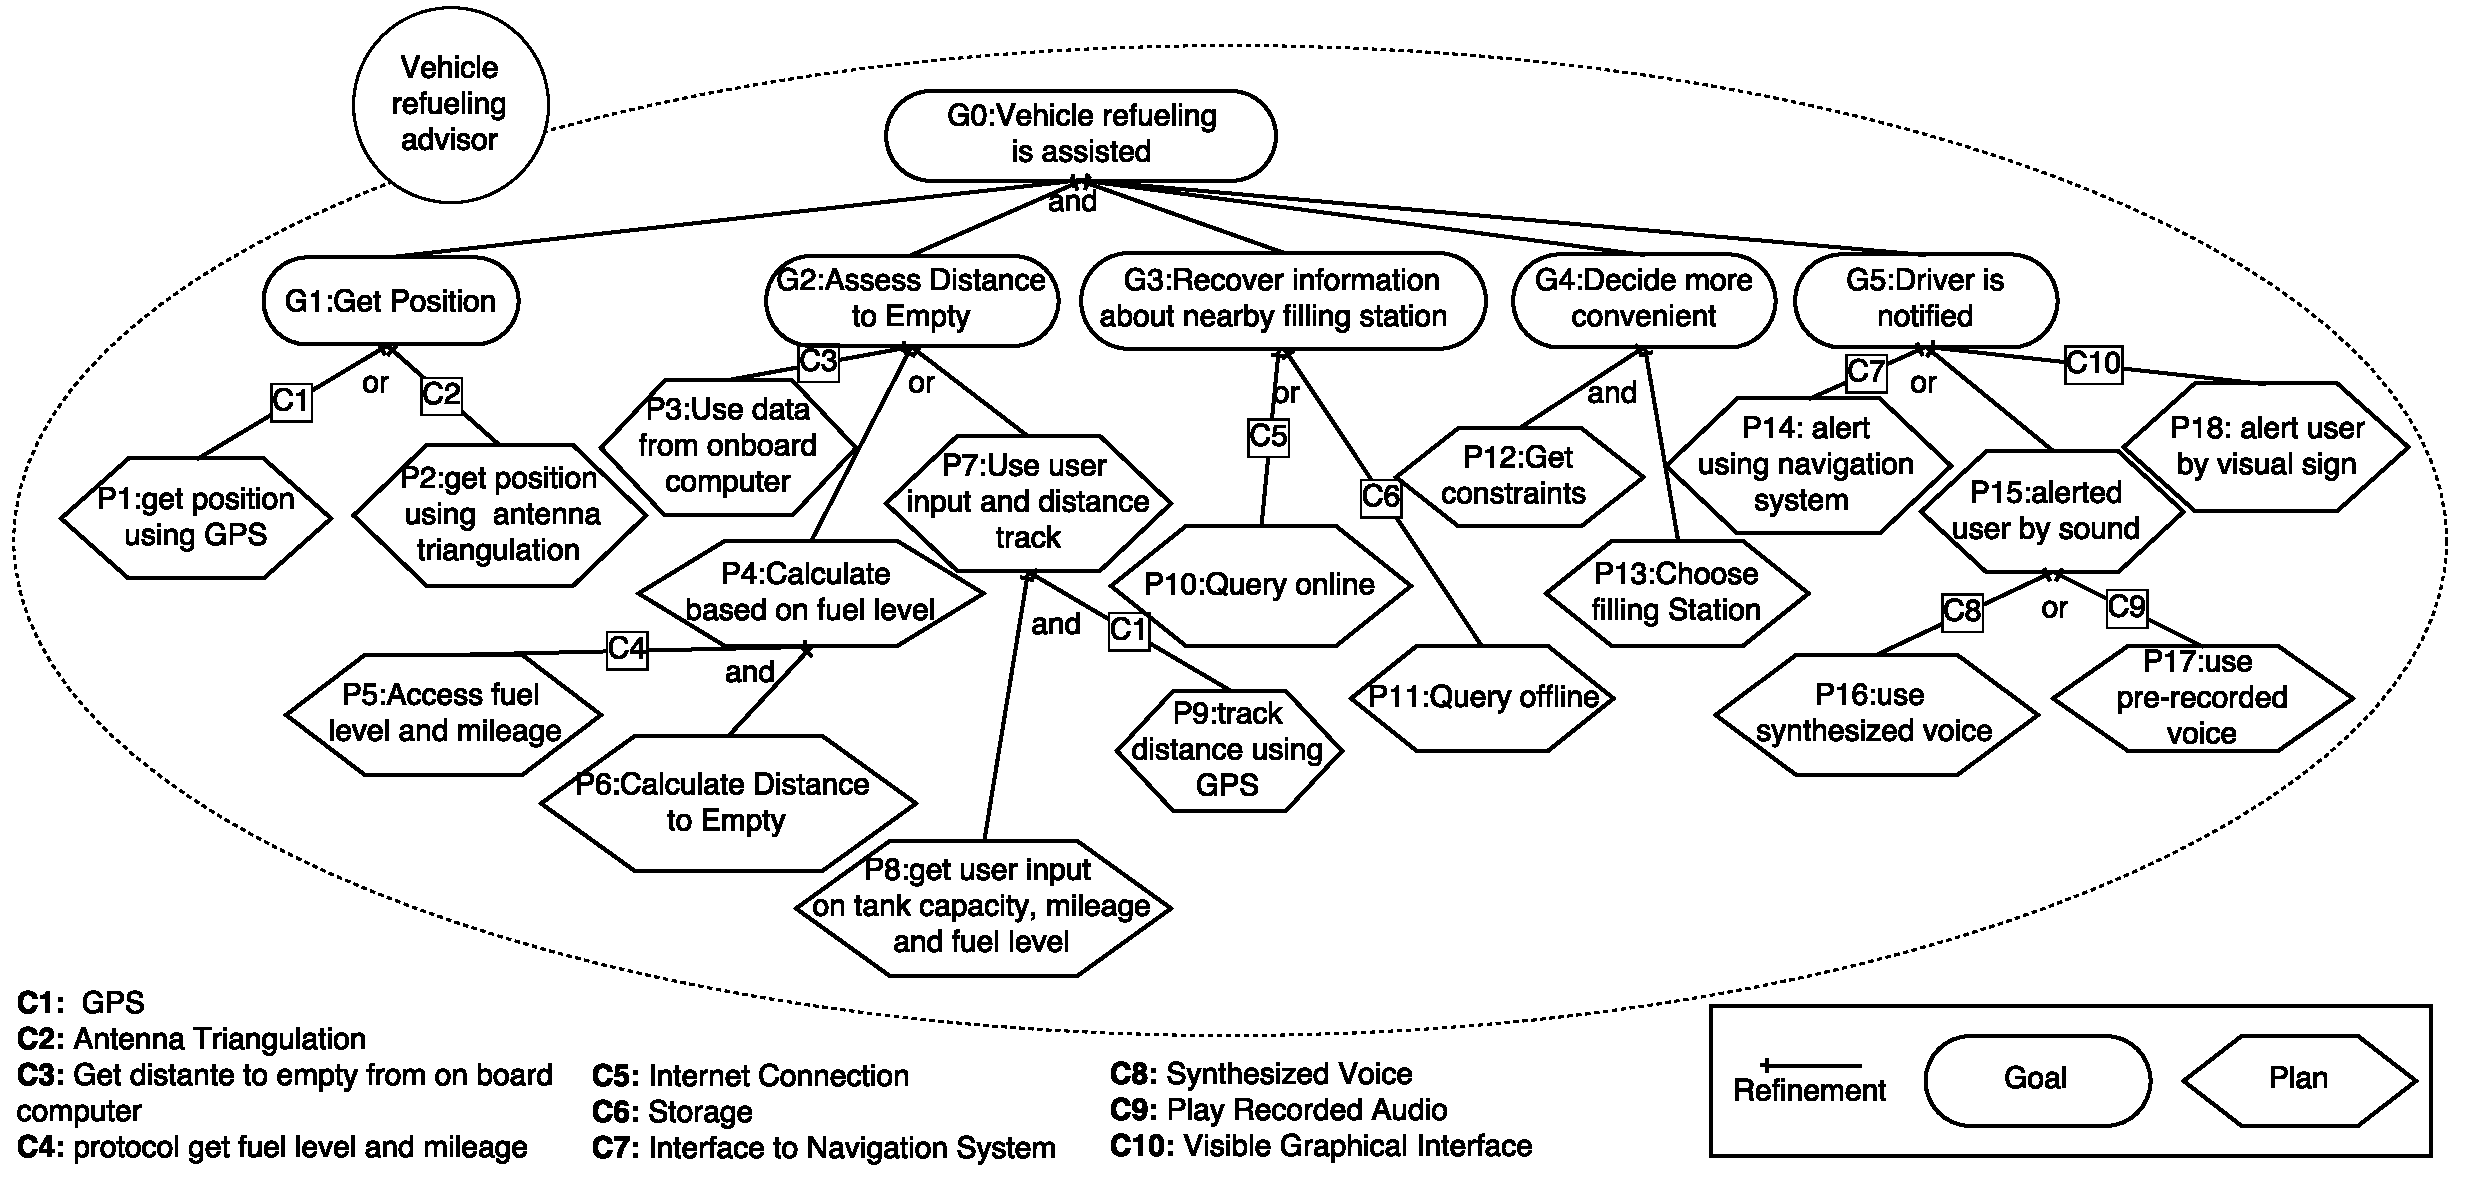
\includegraphics[width=\linewidth]{case_study/goal_model_filling_station_advisor}
 \caption{CGM of the filling station advisor}
\label{fig:goal_model_filling_station_advisor}
\end{figure*}

The CGM presented in Figure~\ref{fig:goal_model_filling_station_advisor} depicts the goals to be achieved by the Filling Station Advisor.
The root objective \emph{G0: Vehicle refueling is assisted} is AND-refined into 5 others objectives G1, G2, G3, G4 and G5. In the Goal modeling semantics it means that in order to achieve the root Goal G0, the agent should achieve the goals G1, G2, G3, G4 and G5.
\emph{G1:Get Position} has a means-end association with P1, P2 and P3. It means that the goal G1 can be achieved by executing that plans. As it is an OR-refinements, it means that G1 can be achieved by successfully executing any of the plans P1, P2 or P3. This OR-refinement introduces a variability to the system, allowing it to achieve to root goals in different ways. The contexts C1 in the association between P1 and G1 means that the Plan P1 is executable if the context C1 holds.
Context conditions on the example are of the type "required context"~\cite{ali_goal-based_2010}. These annotations means that a certain way for achieving (executing) a goal (plan) is applicable if the condition holds for the context.

\begin{figure}[!htb]
 \centering
 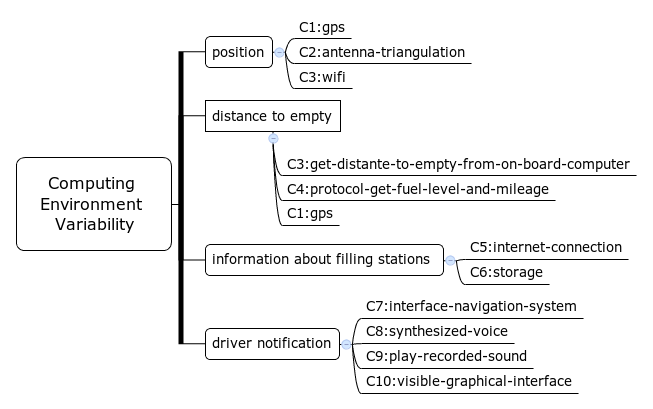
\includegraphics[width=.7\linewidth]{case_study/variability}
 \caption{Variability in the Computing Environment}
\label{fig:variability}
\end{figure}

Figure~\ref{fig:variability} outlines the context space of the target computing environment. It contains variability contexts that are expected to occur in 4 subgoals (G1-G3 and G5) of the application.


\chapter{Background}

\section{Goal Modeling}

Goal-Oriented Analysis is a requirements engineering approach that captures and documents the intentionality behind requirements. Goal-Oriented Requirements Engineering (GORE) approaches have gained special attention as a technique to specify adaptable systems~\cite{morandini_goal-oriented_2009}. Goals capture the various objectives the system under consideration should achieve. In particular, Tropos\cite{bresciani_tropos:_2004} is a methodology for developing multi-agent systems that uses goal models for requirement analysis.
% Wooldridge~\cite{woolridge_introduction_2001} defines Multiagent Systems (MAS) as systems composed of multiple interacting computing elements known as \emph{agents}.
% Agents are computer systems that are capable of autonomous action and interacting with other agents. Jadex is a platform that facilitates development of mult-agent systems~\cite{braubach_developing_2012}.

\subsubsection{The Tropos key concepts}

Tropos uses a modeling framework based on i* \cite{yu_modelling_1996} which proposes the concepts of actor, goal, plan, resource and social dependency to model both the system-to-be and its organizational operating environment \cite{bresciani_tropos:_2004} \cite{morandini_tropos_2014}.

In Tropos, requirements are represented as actors goals that are successively refined by AND/OR refinements. There are usually different ways to achieve a goal, and this is captured in goal models through multiple OR refinements.

Key concepts in the Tropos metamodel are:

\begin{description}%[leftmargin=6em,style=nextline]
  \item[Actor] is an entity that has strategic goals and intentionality

  \item[Agent] is the physical manifestation of an actor.

  \item[Goals] represent actors’ strategic interests. \emph{Hard goals} are goals that have clear-cut criteria for deciding whether they are satisfied or not. \emph{Soft goals} have no clear-cut criteria and are usually used to describe preferences and quality-of-service demands.

  \item[Plans] represent a way of doing something. Plans are concrete actions or procedures that an agent can perform. The execution of a plan can be a means for satisfying a goal or for \emph{satisficing} (i.e. sufficiently satisfying) a soft goal.

  \item[Resource] represents a physical or an informational entity.

  \item[Dependency] it is a relationship between two actors that specify that one actor (the \emph{depended}) has a dependency to another actor (the \emph{dependee}) to attain some goal, execute some plan or deliver a resource. The object of the dependence is the \emph{dependum}.

  \item[Capability] represents both the \emph{ability} of an actor to perform some action and the \emph{opportunity} of doing so.

\end{description}


In Tropos requirements are represented as actors goals that are successively refined by AND/OR refinements. There are usually different ways to achieve a goal, and this is captured in goal models through multiple OR refinements.

Goal models are a traditional requirements tool, as such it must capture the solution space and are not sufficiently detailed to reason about system execution and do not capture information on the status of requirements as the system is executing, nor on the history of an execution~\cite{borgida_requirements_2013}. Traditional goal models can be named design-time goal model (DGM). Dalpiaz et al.\cite{dalpiaz_runtime_2013} describe a method for extending Design-time Goal Models (DGMs) to create Runtime Goal Models (RGM). RGMs can be used to analyze the system's runtime behavior. Other works relate goal models with another dynamic aspects of systems, such as configuration~\cite{yu_goals_2008}, behavior~\cite{dalpiaz_runtime_2013},  probability of achieving success~\cite{mendonca_dependability_2015} and achievability of goals~\cite{pontes_guimaraes_pragmatic_2015}.

Salehie et al.~\cite{salehie_towards_2012} propose a run-time goal model and its related action selection. They model adaptable software as a system that exposes sensors and effectors and proposes a model consisting in \emph{Goals}, \emph{Attributes}, and \emph{Action} for selecting actions that will affect the adaptable software at runtime, giving sensed attributes.
So the adaptation mechanism is to choose the best action given the actual attributes.
It uses explicit runtime goals and makes them visible and traceable.

\subsubsection{Contextual Goal Model}

Contextual Goal Model, proposed in~\cite{ali_goal-based_2010}, captures the relation between system goals and the changes into the environment that surround it. Context goal models extends goal models with context information. Goals and context is related by inserting context conditions on variation points of the goal model. Context Analysis is a technique that allows to derive a formula in verifiable peaces of information (facts). Facts are directed verified by the system, while a formula represents whether a context holds.

Mendonça et al.~\cite{mendonca_dependability_2015} propose GODA: a methodology  for dependability analysis by which the software engineer, at design-time, annotates the goal decomposition in goal model and specify context variables. A special tool generates a formula to evaluate for a given context the probability of achieving a goal at runtime.

This chapter briefly reviews the concepts used throughout this work.


\section{Context-aware Systems}
Context-aware systems are those able to adapt their behavior according to changing circumstances without user intervention. Finkelstein and Savigni~\cite{finkelstein_framework_2001} describe a framework for context-aware services. Their approach is depicted in Figure~\ref{fig:finkelstein_framework}.

\begin{figure}[!htb]
  \centering
  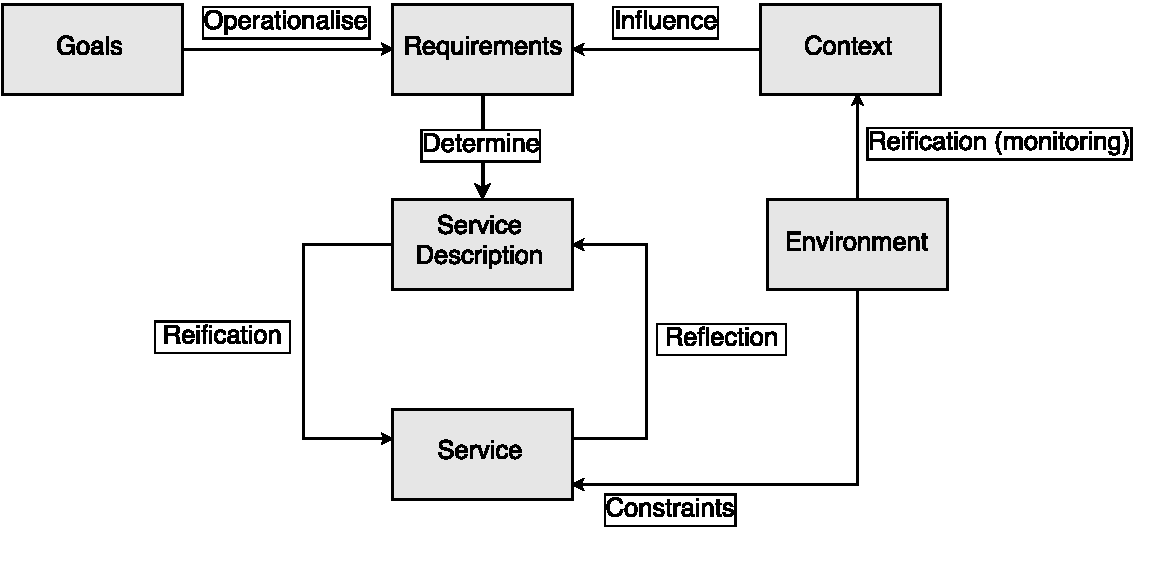
\includegraphics[width=.8\linewidth]{finkelstein_framework}
  \caption{Context-aware services framework by~\cite{finkelstein_framework_2001}}
\label{fig:finkelstein_framework}
\end{figure}

\emph{Environment} is whatever in the world provides a surrounding in which the agent is supposed to operate. The environment comprises such things as characteristics of the device that the agent is expected to operate in.
\emph{Context} is the reification of the environment. The \emph{context} provides a manageable, easily computer manipulable description of the \emph{environment}. A context-aware system should watch relevant environment properties and keep a runtime model that represents those properties. By reasoning about that model the system can change its behavior. A \emph{context} can be either an \emph{activator} of goals or a \emph{precondition} on the applicability of a certain strategy to reach a \emph{goal}.

A \emph{goal} is an objective the system should achieve. It is an abstract and long-term objective of the system. A \emph{requirement} operationalises a goal. It represents a more concrete and short-term objective that is directly achievable through actions performed by one or more agents. \emph{Service description} is the meta-level representation of the actual, real-world service. It should be a suitable formalism that allows services to be compared to requirements in order to identify runtime violations. Service provides the actual behavior as perceived by the user.

A \emph{reflective system} is a system which incorporates structures representing (aspects of) itself. A \emph{causal connection} between a model and a modeled element exists if one of them changes, this leads to a corresponding effect upon the other~\cite{maes_concepts_1987}. Following this approach, the system should keep a causal connection between the service and the description. The system adapts by manipulating the service description.
Following the requirements reflection vision~\cite{bencomo_requirements_2010}, a system should keep software requirements model at runtime, and use such model to drive the system adaptation.

%\input{parts/background/self-}
\section{Software Components}
Heineman define \emph{software component} as a
\say{software element that conforms to a component model and can be independently deployed and composed without modification according to a composition standard}\cite{heineman_component-based_2001}.

Software components is a unit of composition. Software systems are built by composing different components.  Software components must conform to a component model by having contractually specified interfaces and explicit context dependencies only.\cite{szyperski_component_2002}.

A \emph{component	interface} \say{defines a set of component functional properties, that is, a set of actions understood by both the interface provider (the component) and user (other components, or other software that interacts with the provider)}\cite{crnkovic_software_2011}.
A component interface has a role as a component specification and also a means for interaction between the component and its environment.
A \emph{component model} is a set of standards for a component implementation. These standards can standardize naming, interoperability, customization, composition, evolution and deployment.\cite{heineman_component-based_2001}
The \emph{component deployment} is the process that enables component integration into the system. A deployed component is registered in the system and ready to provide services\cite{crnkovic_software_2011}.
\emph{Component binding} is the process that connects different components through their interfaces and interaction channels.

Software architecture deals with the definition of components, their external behavior, and how they interact\cite{kaur_component_2010}. The architectural view of a software can be formalized via an architecture description language (ADL)\cite{medvidovic_classification_2000}.


Component-based software engineering (CBSE) approach consists of building systems from components as reusable units and keeping component development separate from system development\cite{crnkovic_software_2011}.

CBSE is built on the following four principles\cite{crnkovic_software_2011}:
\begin{itemize}
  \item \emph{Reusability}. Components, developed once, have the potential for reuse many times in different applications.
  \item \emph{Substitutability}. Systems maintain correctness even when one component replaces another.
  \item \emph{Extensibility}. Extensibility aims to support evolution by adding new components or evolving existing ones to extend the system’s functionality.
  \item \emph{Composability}. A system should support the composition of functional properties (component binding). Composition of extra functional properties, for example, composition of components’ reliability, is another possible form of composition.
\end{itemize}

\subsection{Component-Based Adaptation}

In the literature was proposed frameworks for architecture and components based adaptation.

Rainbow\cite{garlan_rainbow:_2004} is a framework for self-adaptation architecture based. It keeps an model of the architecture of the system and can be extended with rules to analysis the system behavior at runtime, find adaptation strategies and perform this changes. It separate the functional code (internal mechanisms) from adaptation code (external mechanism) in a schema called external control, influenced by control theory.

MUSIC\cite{rouvoy_music:_2009} project provides a component-based middleware for adaptation that propose to separate the self-adaptation from business logic and delegate adaptation logic to generic middleware. As in our propose it adapts by evaluating in runtime the utility of alternatives, to chose a feasible one (e.g., the one evaluated as with highest utility).

Flashmob~\cite{sykes_flashmob:_2011} is an approach for distributed self-assembly. Different from MUSIC and Rainbow, it handles component-based adaptation in a distributed environment. The self-assembly can be described as: given a set of available components (with various functional and non-functional properties), and a configuration of components which are already running, find a new configuration which works (better) in the changed execution environment (including hardware),
meets new user requirements or takes account of new component implementations~\cite{sykes_flashmob:_2011}. Flashmod uses a three-layer model: goals, management and components proposed by Kramer and Magee~\cite{kramer_self-managed_2007}, extending it to allow distributed agreement in a given configuration.

OSGi\cite{the_osgi_alliance_osgi_2007} is a Java centric platform that allows dynamic bind and unbind of components, usually named bundles. Ferreira et al.\cite{ferreira_-osgi:_2012} proposed a framework for adaptation based on OSGi.

\subsection{From Goals to Components}

Lamsweerde \cite{van_lamsweerde_system_2003} present a method for derive architecture from KAOS goal model. First an abstract draft is generated from functional goals. Secondly, the architecture is refined to meet non-functional requirements such as cohesion.

% Penserini \citep{penserini_design_2007} propose a method for generate agents from goal models.
% Morandini \cite{morandini_towards_2008}
% Tropos - Jadex-BDI}
Pimentel et al. \cite{pimentel_deriving_2012} present a method  using i* models to produce architectural models in Acme. If focus in he development of adaptive systems. First, it transforms a i* model into a modular i* model by means of horizontal transformation. Secondly, it creates an architecture model from the i* modularized model by means of vertical transformation. Architectural design models is made easier by the
presence of actor and dependency concepts.

Yu et al.~\cite{yu_goals_2008} proposed an approach for keep the variability that exists in the goal model into the architecture.
It present a method for creating a component-connector view from a goal model.
A preliminary component-connector view is generated from a goal model by creating an interface type for each goal. The interface name is directed derived from the goal name. Goals refinements result in implementation of components.
If a goal is And-decomposed, the component has as many \emph{requires} interfaces as subgoals.

\begin{lstlisting}
Component G {
  provides IG;
  requires IG1, IG2;
}
\end{lstlisting}

If the goal is OR-decomposed, the interface type of subgoals are the interface type of the parent goal.
%It's the most important patterns as it allow variability at architecture.

\begin{lstlisting}
Component G1 {
  provides IG;
}

Component G2 {
  provides IG;
}
\end{lstlisting}

A component equivalent to the parent goal is generated with a switch.


%TODO Input and outputs are added to the interface.

%TODO Related lower level components can be merged by parametrization.

\subsubsection{Dependency Injection}

Dependency Injection is a pattern that allow for wiring together software components that was developed without the knowledge about it other.~\cite{fowler_inversion_2004}

In OO languages normally you instantiate an Object from a class using an operator (\emph{new} for Java) and a reference to this class. By this the object that is instantiating (the object client) is dependent of the referenced class (the service implementation class). In case of strong typed languages, normally one will get an exception if the referenced class is not present.

So the use of the \emph{new} operator lead to the following disadvantages:
\begin{itemize}
  \item impose compile time dependency between two classes
  \item impose runtime dependency between two classes
\end{itemize}

The basic idea of the Dependency Injection, is to have a separate object, an assembler, that wire together the components at runtime\cite{fowler_inversion_2004}. The client class refer to service using its Interface (the service interface). The assembler can use alternative ways of the \emph{new} to instantiating an object, so that the wiring between client objects and implementation service classes could be postpone to runtime.

By this is we can at runtime:
\begin{itemize}
  \item discover available implementation of a service interface
  \item decide this implementation to instantiate from available implementations
\end{itemize}

Not always this pattern is needed as not always is useful to avoid the reference to a class. But in the context of component-based adaptation it would be specially useful to the decouple client components from service components, allowing runtime reasoning about what implementation to choose.

\begin{figure}[h!]\centering

\begin{tikzpicture}
  \begin{umlpackage}[x=4,y=0]{service interface}
    \umlemptyclass[width=15ex]{IServiceA}
  \end{umlpackage}
  \begin{umlpackage}[x=4,y=-3]{service implementation}
    \umlemptyclass[width=15ex]{ServiceAImpl}
    \umlimpl{ServiceAImpl}{IServiceA}
  \end{umlpackage}
  \begin{umlpackage}[x=0,y=0]{Client}
    \umlemptyclass[width=15ex]{ClientOfServiceA}
    \umlassoc{ClientOfServiceA}{IServiceA}
  \end{umlpackage}
  \begin{umlpackage}[x=0,y=-3]{Assembler}
  \end{umlpackage}
\end{tikzpicture}

\caption{Two components}
\end{figure}

% \subsubsection{Inversion of Control Containers}
% \label{sec:iocc}
%
% It have been used as a core principle in the development of popular frameworks like Sprint and Angular.

\subsection{Development of Self-Adaptive Systems}

For self-adaptive systems (SAS) some activities that traditionally occur at development-time are moved to runtime.  In\cite{andersson_software_2013}
was proposed a process for development of adaptive systems.
Activities performed externally are referred as \emph{off-line activities}, and activities performed internally as \emph{on-line activities}.

The right-hand side of Figure~\ref{fig:sas_lifecycle} depicts a running SAS. At this system we have \emph{Domain Logic} that solves that is responsible for final user goals achievements. And also, \emph{Adaptation Logic}, that is responsible to adapt the system in response to changes in the environment. Adaptation logic implements a control loop in line with the monitor-analyze-plan-execute (MAPE) loop~\cite{kephart_vision_2003}.

The left-hand side of Figure~\ref{fig:sas_lifecycle} represents a staged life-cycle model. Off-line activities work on artifacts such as design model and source code in a product repository and not directly on the running system.


\begin{figure}[!htb]
  \centering
  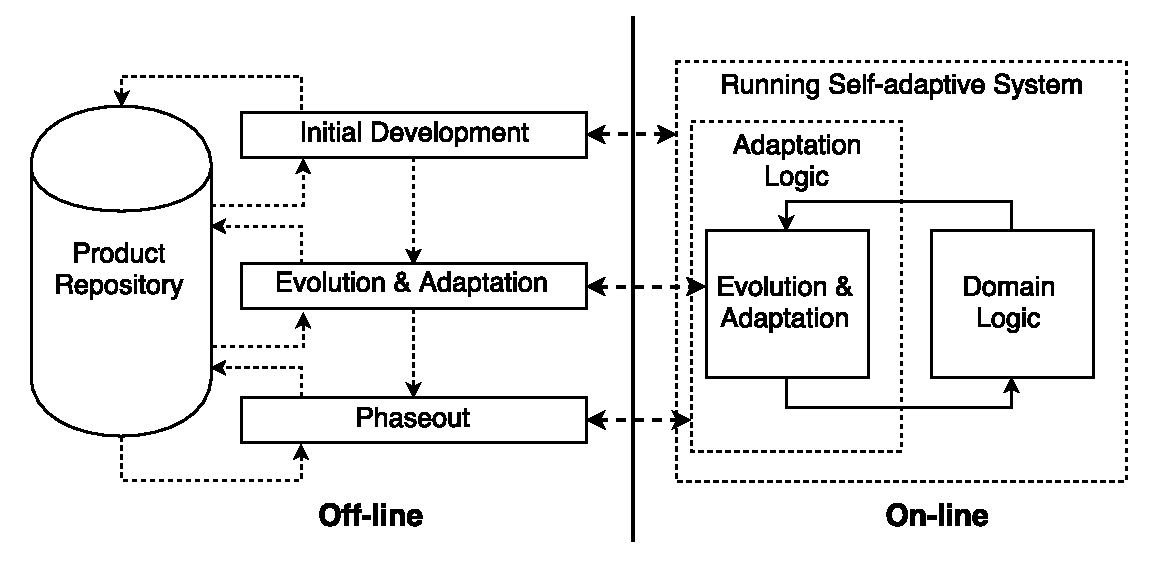
\includegraphics[width=\linewidth]{sas_lifecycle}
  \caption{A Life-cycle model for Self-Adaptation Software System\cite{andersson_software_2013}}
  \label{fig:sas_lifecycle}
\end{figure}

\subsection{Software Deployment}

Software deployment refers to all activities that make a software system available for use\cite{carzaniga_characterization_1998}. These activities result
in the creation and distribution of artifacts,  from the development environment to the target runtime environment. Artifacts are files that package software components and assets. The deployment process can vary depending on the application domain and execution platform. In embedded platforms, the deployment can consist in burning software into a chip. In consumers' personal or business domain, for a desktop platform, the deployment can consist of an installation process with collaboration between a person and a script that automates some steps.
In an enterprise domain, for a web platform it can consist in coping and editing some files in a couple of machines. In many of those scenarios software will be periodically updated, frequently becoming unavailable during the update process.
The complexity of the software deployment can also vary as a function of how much the platform is distributed (i.e. the number of nodes), how much heterogeneous it is, and how much is known about the deployment computing environment at design-time. In a dynamic and heterogeneous environment deployment can be specially complex.

\label{sub:deployment}
\begin{figure}[!htb]
  \centering
  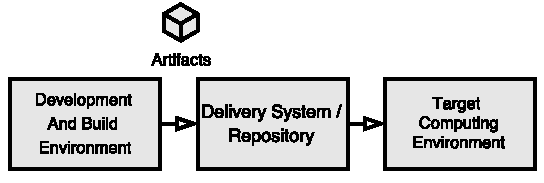
\includegraphics[width=.7\linewidth]{deployment_extended_process}
  \caption{Artifacts Deployment}
  \label{fig:deployment_extended_process}
\end{figure}

Deployment artifacts are the artifacts needed at the deployment environment. Artifacts are built at development and build environment. Built artifacts are move for a delivery system where they can be accessed from the target environment. At deployment the artifacts are moved from the delivery system to the target computing environment. Also, configuration activities can be realized.
In the software industry, a \emph{continuous integration}\cite{humble_continuous_2010} environment applies automation in building and getting components ready to delivery. In such environment if a developer pushes changes to a code repository, components are automatically built and published to delivery system. The build process commonly involves fetching build dependencies, compiling source code, running automated quality control (tests and static analysis) and packaging components into artifacts. Artifacts are published if target quality policies are met.
%dependency manager
Fundamental to continuous integration environments are \emph{Package Management Systems} tools, such as Maven\cite{apache_apache_2016} for Java platform. These tools simplify the management of software dependencies~\cite{spinellis_package_2012}. Such tools ensure that development team members are working with same dependencies that are used in the build environment.
%Sistemas de Gereencia de Pacotes simplificam o processo de instalacao de dependencias. Um pacote contem em um formato padronizado codigo ou codigo compilado, juntamente a sua documentacao e metadados [7]. Os metadados normalmente incluem nome, versao e especificacao de instalacao. Sistemas de Gerencia de Pacotes gerenciam a obtencao e instalac ̧a  ̃ o de dependˆ encias de forma automatizada, com o m ́ınimo de interac ̧ a  ̃o com o usu ́ ario e consequentemente favorecem a reprodutibilidade.
%build manager

Research in software configuration and deployment, has focused on responding to dynamisms in a known environment. This could be costs and failures in a cloud environmet \cite{ferreira_leite_user_2014}, changes in managed resources \citep{gunalp_rondo_2015}, and changes in the context of operation~\cite{bencomo_dynamically_2008}.

\emph{Continuous delivery}\cite{humble_continuous_2010} extends the continuous integration environment, moving components from the delivery system to a target computing environment with none or minimum human intervention.

In the industry, package managers such as aptitute/apt-get(Debian based Linux distributions)\cite{aoki_debian_2016}, yum (Red Hat based Linux distributions)\cite{svistunov_red_2016}, Homebrew (MacOS)\cite{homebrew_homebrew_2016} and Chocolatey (Windows)\cite{chocolatey_chocolatey_2016} are capable of solving dependencies and deploying software. They require that a managed application declare their dependencies by name and version. DevOps\cite{bang_grounded_2013} is a movement in software industry that advocates that all configuration steps needed to configure the computing environment should be written as code (\emph{infrastructure as code}), following best practices of software development. That movement favors the documentation, reproducibility, automation and scalability.
%Tools such as Puppet and Chef are used by devopers to manage infrastructure.
DevOps allows for management of scalable computing environments. It can offer a significant advantage for enterprise environment in relation to manual approaches in which system administrators configure the system by manually following configuration steps. Current continuous integration/delivery and DevOps practices are not sufficient for highly dynamic and heterogeneous target computing environments; they require that highly specialized system administrators to analyze the environment and create environment configuration descriptors.
%% Deployment in IoT??


%\section{Self-Adaptive Systems}


Self-adaptive systems have been accepted as a promising approach to tackle context change. Self-adaptivesses is an approach in which the system
\textit{"evaluates its own behavior and changes behavior when the evaluation indicates that it is not accomplishing what the software is intended to do, or when better functionality or performance is possible."}\cite{laddaga_self_1997}.

%kramer et al. dream

Self-adaptive software aims to adjust various artifacts or attributes in response to changes in the self and in the context of a software system\cite{salehie_self-adaptive_2009}.

A key concept in self-adaptive systems is the awareness of the system. It has two aspects\cite{salehie_self-adaptive_2009}:
\begin{itemize}
   \item \textit{self-awareness} means a system is aware of its own states and behaviors.
   \item \textit{context-awareness} means that the system is aware of its context,
\end{itemize}

Schilit et al.\cite{klein_survey_2008} define \textit{context} as \say{the sufficiently exact characterization of the situations of a system by means of perceivable information that is relevant for the adaptation of the system}.

Schilit et al.\cite{klein_survey_2008} define \textit{context adaptation} as \say{a system’s capability of gathering information about the domain it shares an interface with, evaluating this information and changing its observable behavior according to the current situation}.


% laddaga1997: it should relies on software informed about its mission and about its construction and behavior.  This implies that the software has multiple ways of accomplishing its purpose, and has enough knowledge of its construction to make effective changes at runtime.

% Such software should include functionality for evaluating its behavior and performance, and the ability to replan and reconfigure its operations in order to improve its operation.  Self adaptive software should also include a set of components for each major function, along with descriptions of the components, so that components of systems can be selected and scheduled at runtime, in response to the evaluators.

% It also requires the ability to impedance match input/output of sequenced components, and the ability to generate some of this code from specifications. In addition, we seek this new basis of adaptation to be applied at runtime, as opposed to development/design time, or as a maintenance activity.


% mape-k

% different approaches ref salehie

% challenges

%
% A self-managed software architecture is one in which components automatically configure their interaction in a way that is compatible with an overall architectural specification and achieves the goals of the system\cite{kramer_self-managed_2007}.

% Component Control
% include the capability to support component creation, deletion and interconnection.

% include facilities to report the current status of components to higher layers and also include the capability to support component creation, deletion and interconnection.
% adjust the operating parameters of components
% self-tuning algorithms, event and status reporting to higher levels and operations to support modification – component addition, deletion and interconnection.
% situation is met that the current configuration of components is not designed to deal with, this layer detects this failure and reports it to higher layers.



% Change Management

% Goal Management

%\chapter{Self-adaptability Architectures}

%\section{Cloud Computing}
%\section{Goal-oriented requirements engineering}

Goal-oriented requirements engineering (GORE) is concerned with the use of goals for eliciting, elaborating, structuring, specifying, analyzing, negotiating, documenting, and modifying requirements\cite{van_lamsweerde_goal-oriented_2001}.

GORE models are the main tool used by system analysts and stakeholders to reason about the system requirements. Goal modeling represents a shift in relation to traditional software development approaches as it focus on stakeholder goals and states that the system needs to achieve and not in how it achieves it\cite{ali_goal-based_2010}. Goal models are graphs representing AND/OR-decomposition of abstract goals down to operationalisable leaf-level goals. \cite{morandini_operational_2009}

A goal is an objective the system under consideration should achieve. \cite{van_lamsweerde_goal-oriented_2001}

\section{TROPOS}
Tropos\cite{bresciani_tropos:_2004} is a methodology for develop multi-agent systems that uses goal models for requirement analyses. Tropos encompasses the software development phases, from Early Requirements to Implementation and Testing.

\subsection{The Tropos key concepts}

The methodology adopts the i* \cite{yu_modelling_1996} modeling framework, which proposes the concepts of actor, goal, task, resource and social dependency to model both the system-to-be and its organizational operating environment\cite{bresciani_tropos:_2004}. In more recent publication \cite{morandini_tropos_2014} about the Tropos modeling framework the concept of \textit{task} was renamed to \textit{plan}.

The following are the key concepts in the Tropos metamodel\cite{morandini_tropos_2014}:

\begin{itemize}
    \item Actor: an entity that has strategic goals and intentionality
    \item Goals: it represents actors’ strategic interests. \texit{Hard goals} are goals that have clear-cut criteria for deciding whether they are satisfied or not. \textit{Softgoals} have no clear-cut criteria and are normally used to describe preferences and quality-of-service demands.

    \item Plan: it represents, at an abstract level, a way of doing something. The execution of a plan can be a means for satisfying a goal or for \textit{satisficing} (i.e. sufficiently satisfying) a softgoal.

    \item Resource: it represents a physical or an informational entity.

    \item Dependency: its a relationship between to actors that specify that one actor (the \textif{depended}) have a dependency to other actor (the \textit{dependee}) to attain some goal, execute some plan or deliver a resource. The object of the dependence is the \texit{dependum}.

    \item Capability: it represents both the \textit{ability} of an actor to perform some action and the \textit{opportunity} of doing this.

\end{itemize}

% TODO Runtime goal models

%\section{Dependability}
Dependability can be defined as the ability of a system to avoid faults in its services
that (1) are more frequent or (2) more severe that is acceptable. Or as the characteristic of a system to be justifiably trusted.

A common terminology used for system deviations as the following: \cite{avizienis_basic_2004}

\begin{itemize}
  \textbf{failure}: or \textif{service failure} is a perceived deviation from the correct service provided by a system.
  \textbf{error}: is a deviation of correct internal system state that can lead to its subsequent failure.
  \textbf{fault}: is the adjudged or
hypothesized cause of an error
\end{itemize}

Dependability include the following attributes:\cite{avizienis_basic_2004}
\begin{itemize}
  \item \textbf{availability}: readiness for correct service.
  \item \textbf{reliability}: continuity of correct service.
  \item \textbf{safety}: absence of catastrophic consequences on the
user(s) and the environment.
  \item \textbf{integrity}: absence of improper system alterations.
  \item \textbf{maintainability}: ability to undergo modifications and repairs.
\end{itemize}


Many means have been developed of how attain the attributes of dependability. This means can be classified as:

\begin{itemize}
  \item \textbf{Fault prevention} means to prevent the occurrence or introduction of faults.
  \item \textbf{Fault tolerance} means to avoid service failures in the presence of faults.
  \item \textbf{Fault removal} means to reduce the number and severity of faults.
  \item \textbf{Fault forecasting} means to estimate the present number, the future incidence, and the likely consequences of faults.
\end{itemize}


% TODO dependability in face of uncertainty

\section{Attain Dependability at Runtime }
To keep dependability in face of uncertainty in the deployment environment some techniques was proposed for runtime analysis at runtime.

Felipe et al\cite{guimaraes_framework_2013} propose a method of fault-tolerance for a scientific workflow execution in grid.

Alessandro Leite \cite{ferreira_leite_user_2014} propose a fault tolerance schema for cloud deployment based on which a fault instance in the cloud is monitored and in case of failure the instance can be restarted or terminated and them a new instance created.

Danilo et al\cite{mendonca_dependability_2015} propose a methodology for fault forecasting by which developer, at design time, annotate the goal decomposition in goal model and specify context variables. A special tool generate a formula for, given a context, evaluate the probability of achieve a goal at runtime.

% Pessoa et al \cite{pessoa_dependable_2015} propose a ... with and evaluate it with focus on safety ...


 % reduce redundancy

%\section{Model Checking}


\chapter{Related Work}
%\section{Self-adaptability}
%\section{Open-Systems}

%\chapter{Model at Runtime}

%\section{Component Based}

Architectural or component-based modes represent the system as

as a gross composition of components, and their properties of interest\cite{garlan_rainbow:_2004}

considerar the system as

%\section{Dependability}
%\input{related/ecs}
%\section{Related Work}
\label{related}


Rainbow is a framework for self-adaptation architecture based\cite{garlan_rainbow:_2004}. It keeps an model of the architecture of the system and can be extended with rules to analyses the system behavior at runtime, find adaptation strategies and perform this changes. It separate the functional  code (internal mechanisms) from adaptation code (external mechanism) in a schema called external control, influenced by control theory. \cite{garlan_software_2009}
Different from our proposal Rainbow don't enforce an specific architecture what could be special useful in case of retrofitting a pre-existent systems. Different from our proposal its not goal-oriented an for the best of our knowledge there is no work on how to map goals to  components.

MUSIC project provides a component-based middleware for adaptation that propose to separate the self-adaptation from business logic and delegate adaptation logic to generic middleware. As in our propose it adapts buy evaluate in runtime the utility of alternatives, to chose a feasible one (e.g., the one evaluated as with highest utility)\cite{rouvoy_music:_2009}. As Rainbow, MUSIC is not goal-oriented.
% Yet it provide means of supporting seamless configuration of component frameworks based on local, remote components and services.

Salehie et al. \cite{salehie_towards_2012} propose a run-time goal model and its related
action selection. It models adaptable software as a system that exposes sensors and effectors and  proposes a model consisting in Goals, Attributes and Action for selecting actions that will effect the adaptable software at runtime, giving sensed attributes.
So the adaptation mechanism is to choose the best action given the actual attributes.
As this work it uses explicit runtime goals and make them visible and traceable.
Different from it we use a more symmetric approach that can allow for functional
and adaptation management.
%The validation is make on simulated environment.

Günalp et al. \cite{gunalp_autonomic_2012} propose a middleware for pervarsive software with autonomic capabilities. The approach is service based. It proposes a component written in a custom language and the use of components repository that allows the discovery on new sensors. The system present a support for adaptability by using policies.
% Different from this work it did not present support for collaboration/delegation of goals to another peers. It don't allow for runtime incorporation of adaptation strategies, also.


%\section{Conceptual Model}
\label{conceptual_model}

An agent, in multi-agent systems, is an unit in the system capable of take independent actions. In your conceptual model an agent is an independent computational unit that manages its own resources (CPU, memory, disk, sensors, etc).

\begin{figure}
  \centering
  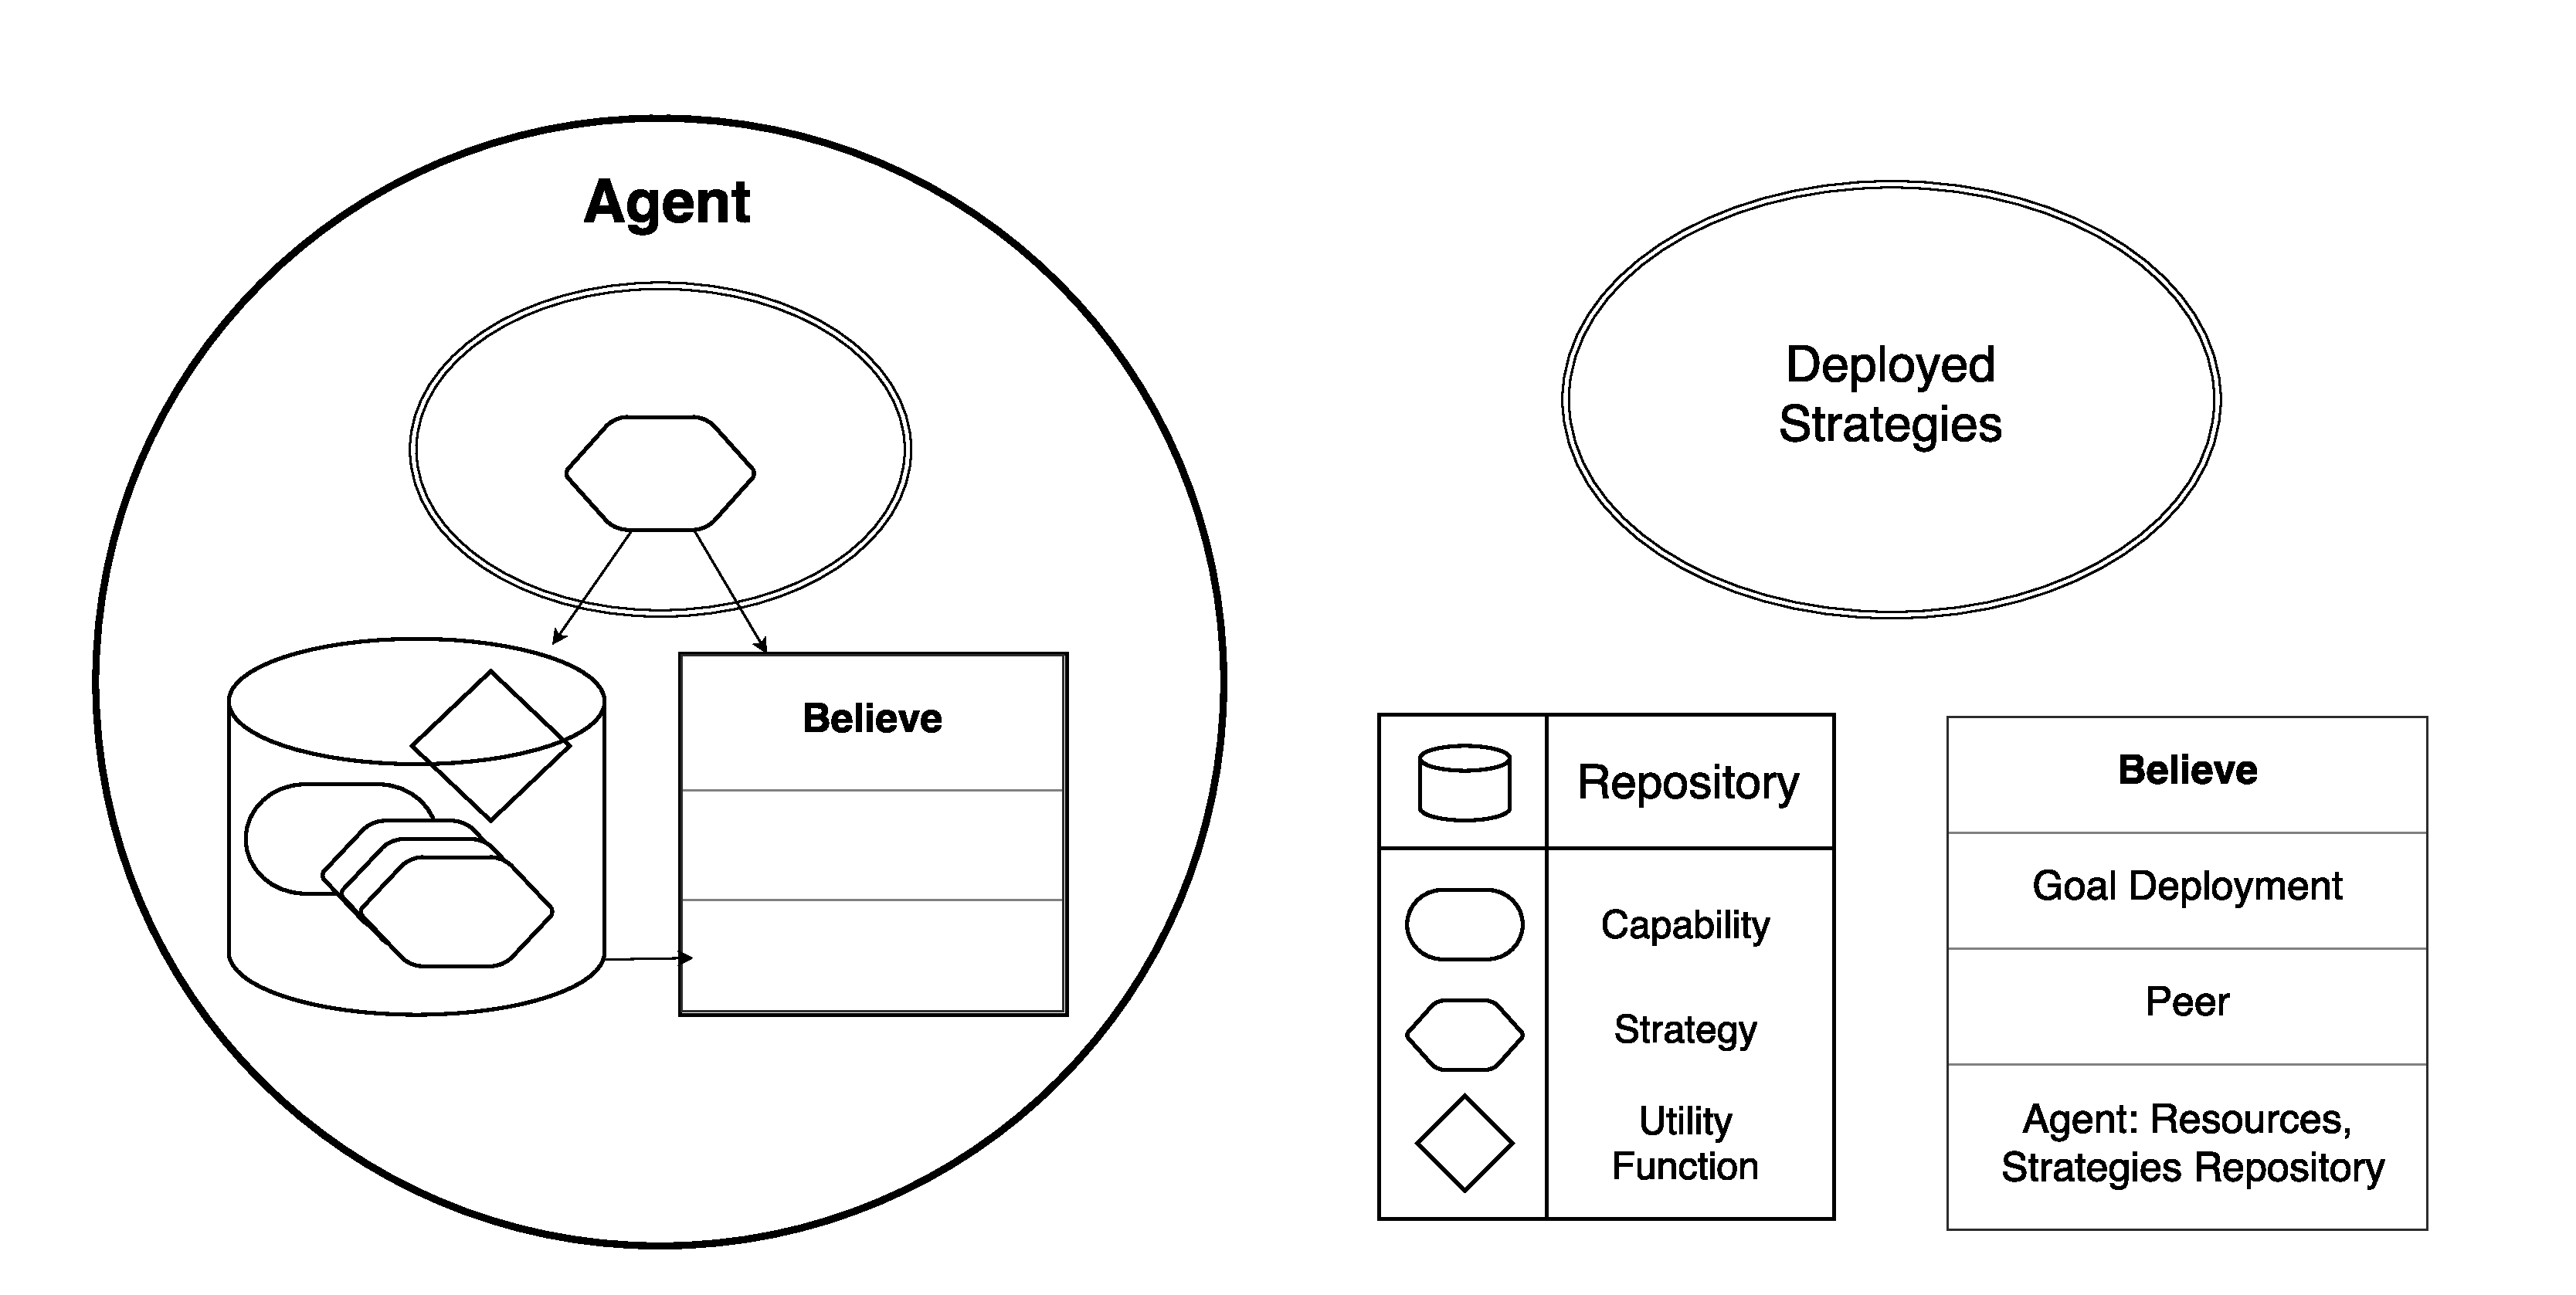
\includegraphics[width=\linewidth]{goalp-agent-repo-rcm-depl}
  \caption{The Agent}
  \label{fig:goalp-agent}
\end{figure}



The system requirements will be represented by 'capacities'. Capacities are what goals a system can accomplish in a goal-model semantics. The system 'capacities' are implemented by 'strategies'.
The 'strategy' is both a mean of achieving a goal (as in GORE) and a component in the architecture. By this we aim at creating an appropriate abstraction to allow composable adaptable architecture while keeping the traceability between the requirements and implementation at runtime.

An agent in the system has a repository of strategies that had all its runnable code. The agent have a model of that repository that it can use for reason about its capacities. The agent can also insert and remove strategies from its repository.

\begin{itemize}
  \item \textbf{Capability}: description of a kind of goal that an agent can perform.   Its an interface description in the architecture. (e.g SUM a and b)
  \item \textbf{Goal Instance}: an actual instance of an objective for a given data set. (e.g SUM 2 and 3)
  \item \textbf{Strategy}: a strategy is a 'Capability Goal' alternative implementation (e.g (SUM,a,b) => {a+b}). Its also a module in the architecture.
  \item \textbf{Strategies Repository}: repository of know strategies
  \item \textbf{Utilitarian Function}: select strategies based on context
  \item \textbf{Runtime Context Model}: data structures that represent the knowledge of the agent.
\end{itemize}

In the proposed model an actor achieve a goal by \emph{deploying a strategy}. For instance the deployment of goals is a capability itself, as follows:

\begin{figure}
  \centering
  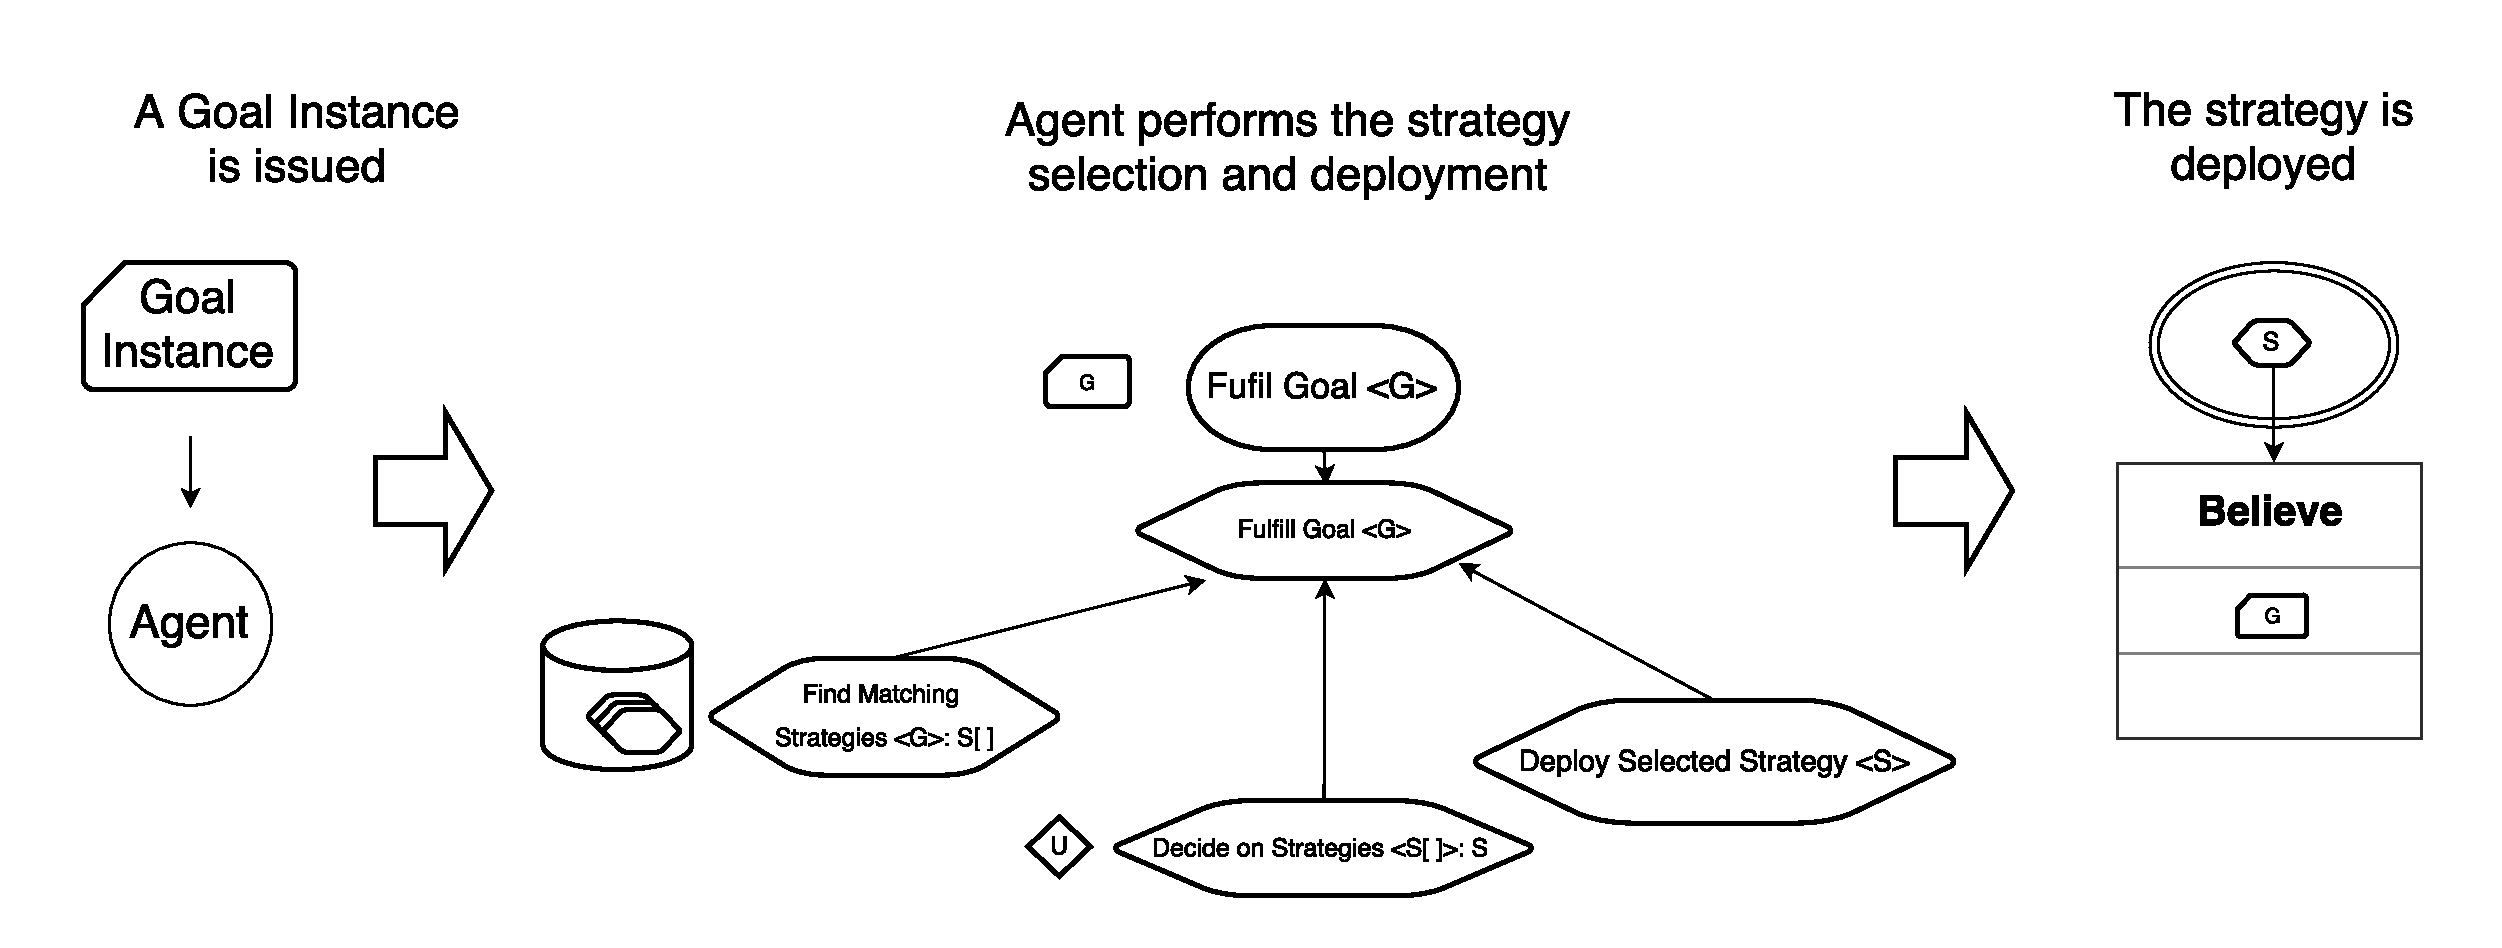
\includegraphics[width=\linewidth]{strategy_deployment}
  \caption{The deployment of a strategy}
  \label{fig:agent_composition}
\end{figure}

\begin{itemize}

\item \textbf{<Fulfill Goals> Goal} the capability of fulfill generic goals.

\item \textbf{<Utilitarianlly Fulfill Goals> Strategy } strategy to fulfill goals by selecting available strategies and evaluating them with an utilitarian function. Consist of 3 sub-goals:
  \begin{itemize}
    \item Find Matching Strategies
    \item Decide on Strategies
    \item Deploy the Selected Strategy
  \end{itemize}
\end{itemize}

And the following three strategies implement the previous 3 goals.

\begin{itemize}
  \item \textbf{<Find Local Matching Strategies> Strategy} accomplish <find matching strategies>
  return the list of matching strategies. An matching strategy is any strategy that implement the goal interface.

  \item \textbf{<Utilitarianlly Select a Strategy> Strategy} accomplish <Utilitarianlly Fulfill Goals>
  use a pre-configured utilitarian function that analyses strategies metadata and select a strategy.

  \item \textbf{<Deploy Strategy> Strategy} accomplish <Deploy Strategy>.
  Consist of call the strategy code for the 'goal issue' runtime context model.
\end{itemize}

%
% \section{Resources}
%
% \section{Strategy Declaration}
%
%
% \section{Fault Model}
% Consistent/Inconsistent Failure
%
% Agent failure
%
% Resource failure
%
% Strategy failure

% Related Work(0.5p)
% \section{Related Work}
% \label{sec:related}

In this chapter, we will highlight the most closely related
work.
%Before we describe Goalp in detail, we review relate work and the background terms necessary to understand our approach.


% Other approaches for context-aware systems threat context-requirements as a tupla (context, requirement)\cite{knauss_acon:_2016}. These approaches handle the runtime of a context-requirements. When the context is valid the requirements apply. In this work, we handle the deployment view. Therefore, we need a different view: if the context is possible, the requirement should be satisfiable.

% Research in software configuration and deployment, has focused on respond to dynamisms in a known environment. This could be costs and failures in a cloud environmet \cite{ferreira_leite_user_2014}, changes in managed resources \citep{gunalp_rondo_2015}, and changes in the context of operation \cite{bencomo_dynamically_2008}.

% In the literature, there are proposals that tackle the problem of handling changes at system context~\cite{knauss_acon:_2016}. These proposals focus on the system external context, reasoning about known facts about the external managed world and how it affects the systems goals.

Bencomo et al.~\cite{bencomo_dynamically_2008} uses a SPL approache to adaptation. It  associates an architecture variability model with an environment variability model. The environment variability is modeled as a transition system. The structural variability is responsible for the system adaptation. A configuration or a product is a set of component selected. A configuration is associated with states in the environment variability model. Unlike our approach, their focus is on the adaptation in the configuration at runtime but not in the deployment. \citep{mizouni_framework_2014} uses a feature model associated with context requirements.

%In order to allow a decentralized evolution of the system, Goalp do not rely on a centralized model created at design-time. Instead, metadata present into artifacts contained into an artifact repository is used. This allows third party developers to provide software components with different restrictions of the original developer, creating more variability and in consequence, allowing the application to be executed in a more broad range of devices.
Leite et al.~\cite{ferreira_leite_user_2014} proposes an approach for automatic deployment on inter-cloud environments. It relies on abstract and concrete features models and constraint satisfaction problem solver to create a computing environment using resources distributed across various clouds.
It integrates a self-healing schema for cloud deployment based on which virtual machines in the cloud are monitored and in case of failure the machine can be
restarted or terminated and them a new one created.
The approach is specific to cloud environments and require instantiating at design-time a model with knowledge about the environment.
It also strongly depends on design-time created scripts to realize the deployment of an application, which limits the autonomy of the approach, specially in a unknown environment.

Gunalp et al.~\citep{gunalp_rondo_2015} presents an approach for automatic deployment, in which the deployment specialist specifies the system deployment in terms of resources and desired target states of this resources. The approach follow preset strategies to keep the managed software resources in the specified states. They uses a low level model to driven the adaptation (target states and strategies to change states). Differently, our approach uses a goal-model with is a more abstract model.

Angelopoulos et al.~\cite{angelopoulos_capturing_2015} present an approach to handle  variability at three different dimensions: goals, behavior and architecture. Variability can occur at goals dimension as an OR-refinement or context selection; at behavior dimension as different plans flows; and in architecture with variability of components and implementations. However, their approach does handle variability at deployment.

% Asadie et al.~\cite{asadi_goal-oriented_2011} relates Goal-Oriented requirements and feature models for the development of SPL using a goal-oriented approach. In the described approach Goal-Models complement feature-models providing a mechanism to choose a set of features from stakeholder intentions.

Ali et~al.\cite{ali_requirements-driven_2014} explore the optimization of the deployment for a given context variability space in which the system will be deployed. CGM was used to represent aspects of the environment related to the space of solution, that were to be analyses at design-time. This analyses at design-time can be used to evaluate which alternative strategy to implement.
It differ from our work in which we explore the context of the computing environment. Our approach analysis allow for choosing between components already implemented at deployment time. Both approaches could be used in tandem, as they use the same model (CGM) and provides different analysis.

% GOAL-Architecture
% In this work we present a Goal-Architecture view. Such view was presented in the literature. STREAM-A\cite{pimentel_deriving_2012} create specialized agents. We create components. Components are not agents as they do not have autonomy, instead they are means of achieving a goal.
% Different for other works

% Must of these approaches ignores variability in the computing environment, the underline computing resources that form the infrastructure for executing the system software. None of them solve the problem of software development for a highly variable environment from different software providers.
% Our approach focus on how move components to target environment.

In the industry, package managers such as aptitute/apt-get(Debian based Linux distributions), yum (Red Hat based Linux distributions), Homebrew (MacOS) and Chocolatey (Windows) are capable of solve dependencies and deploy software. They require that a managed application declare their dependencies by name and version. In our approach, differently, the dependencies are declared in terms of interfaces for which implementations are required, not specific implementations. For example, in our case study, the advisor root strategy declares that it requires any artifact that provides \emph{Get Position} goal achievement, but not a specific artifact is required.
This requirement declaration, in terms of interface, associated with context conditions allow for a more flexible dependency resolution at deployment-time.

Table~\ref{table_related_works} characterizes and compares research related to Goalp.

\begin{table*}[t]
\centering
\caption{Comparing characteristic properties of selected approaches related to Goalp}
\label{table_related_works}
\begin{tabular}{|p{4cm}|p{1.75cm}|p{1.75cm}|p{1.75cm}|p{1.75cm}|}
\hline
Work by &
   Goal  \newline Oriented &
    Handle  \newline Heterogeneity &
    Autonomic  \newline  Deployment \newline Planning \\ \hline

Ali et al.\citep{ali_requirements-driven_2014} & Yes & No & No \\ \hline
Angelopoulos et al. \cite{angelopoulos_capturing_2015} & Yes & No & No \\ \hline
Mizouni et al. \citep{mizouni_framework_2014} & No & Yes & No \\ \hline
Leite et al. \citep{ferreira_leite_user_2014}  & No & Yes & No \\ \hline
Gunalp et al.\citep{gunalp_rondo_2015} & No & Yes  &  No\\ \hline
Goalp & Yes & Yes & Yes \\ \hline
\end{tabular}
\end{table*}


% While package mangers such as aptitude and RPM can get components and handle some variabilities, e.g CPU architecture, they are not adaptive, so they not handle changes in the computing environment at runtime. They favor reuse at a library level. We propose reuse at component level.


\chapter{Filling Station Advisor}
% Proposal (3.5p)
\section{Motivating Example: The Filling Station Advisor}
\label{sec:case_study}

In this work, we use a filling station advisor application as a case study to exemplify the application of our approach.
Filling station here refers to a place where the car can be refueled or recharged (gas station/petrol or charge station). The main goal of the filling station advisor is to give directions to a driver about nearby filling stations that can be reached conveniently. By convenient we mean that certain conditions for the chosen station have to be fulfilled as well as user preferences are considered. Examples of conditions are: fuel is compatible with the vehicle; station is located inside the vehicle distance-to-empty. Examples of users preferences are: low price, low number of stops, small deviation from an actual route, and station reputation.

In this work, we will focus on the challenge of handling the computing variability when developing such application. To maximize the utility, the filling station advisor should be able to run in a broad range of devices like smart-phones and car navigation systems. Each of such devices can have a different set of resources that can be used to find a convenient filling station according to the user preferences. For example, in a scenario (s1) where a human driver is using the application with a smart phone, we could use the GPS resource to track the position and the distance since the last refueling; the Internet connection to find nearby filling stations; the device text-to-speech engine to create a voice message to alert the driver when he is passing by a convenient filling station. In another scenario (s2), in which the application is running in onboard computer of an Internet connected self-driving car, we could use a more precise distance-to-empty data from onboard computer, and replace the text-to-speech notification with a system call to the vehicle self-driving system advising the next filling station stop.

The main goal of the application is refined in the following five goals, each one with its own computing resources requirements:

\begin{description}
  \item[Get Position:]
  the system should identify the vehicle position using an available positioning system. To fulfil such goal, a GPS or cell antenna triangulation could be used.

  \item[Assess Distance to Empty:]
  the system should make use of the best available data about the vehicle distance to empty. It could be: access a standard or proprietary interface within the vehicle that provides the data directly as calculated by the onboard computer; use an interface to access data about fuel level and mileage average and calculate the distance to empty; use user input about tank capacity, vehicle mileage, and keep track of distance traveled since the last time the tank was felt completely.

  \item[Recover information about nearby filling stations:]
  the system should recover information about nearby filling stations by: querying available services on the Internet, if connection and servers are available. Otherwise, the system should use previously cached results.

  \item[Decide on the most convenient filling station:]
  Based on position, distance to empty and nearby gas stations, the application should try maximize some user preference, it being low cost, low number of stops, prioritize an automotive fuel brands or gas station reputation.

  \item[Notify Driver:] the application should decide when and how to notify the driver with advices on when to stop in a filling station. The notification could be integrated with an active navigation system if such an interface exists; otherwise it should notify the driver using text-to-speech engine, a pre-recorded voice audio, or on-screen notification.

\end{description}


\begin{figure*}[!htb]
 \centering
 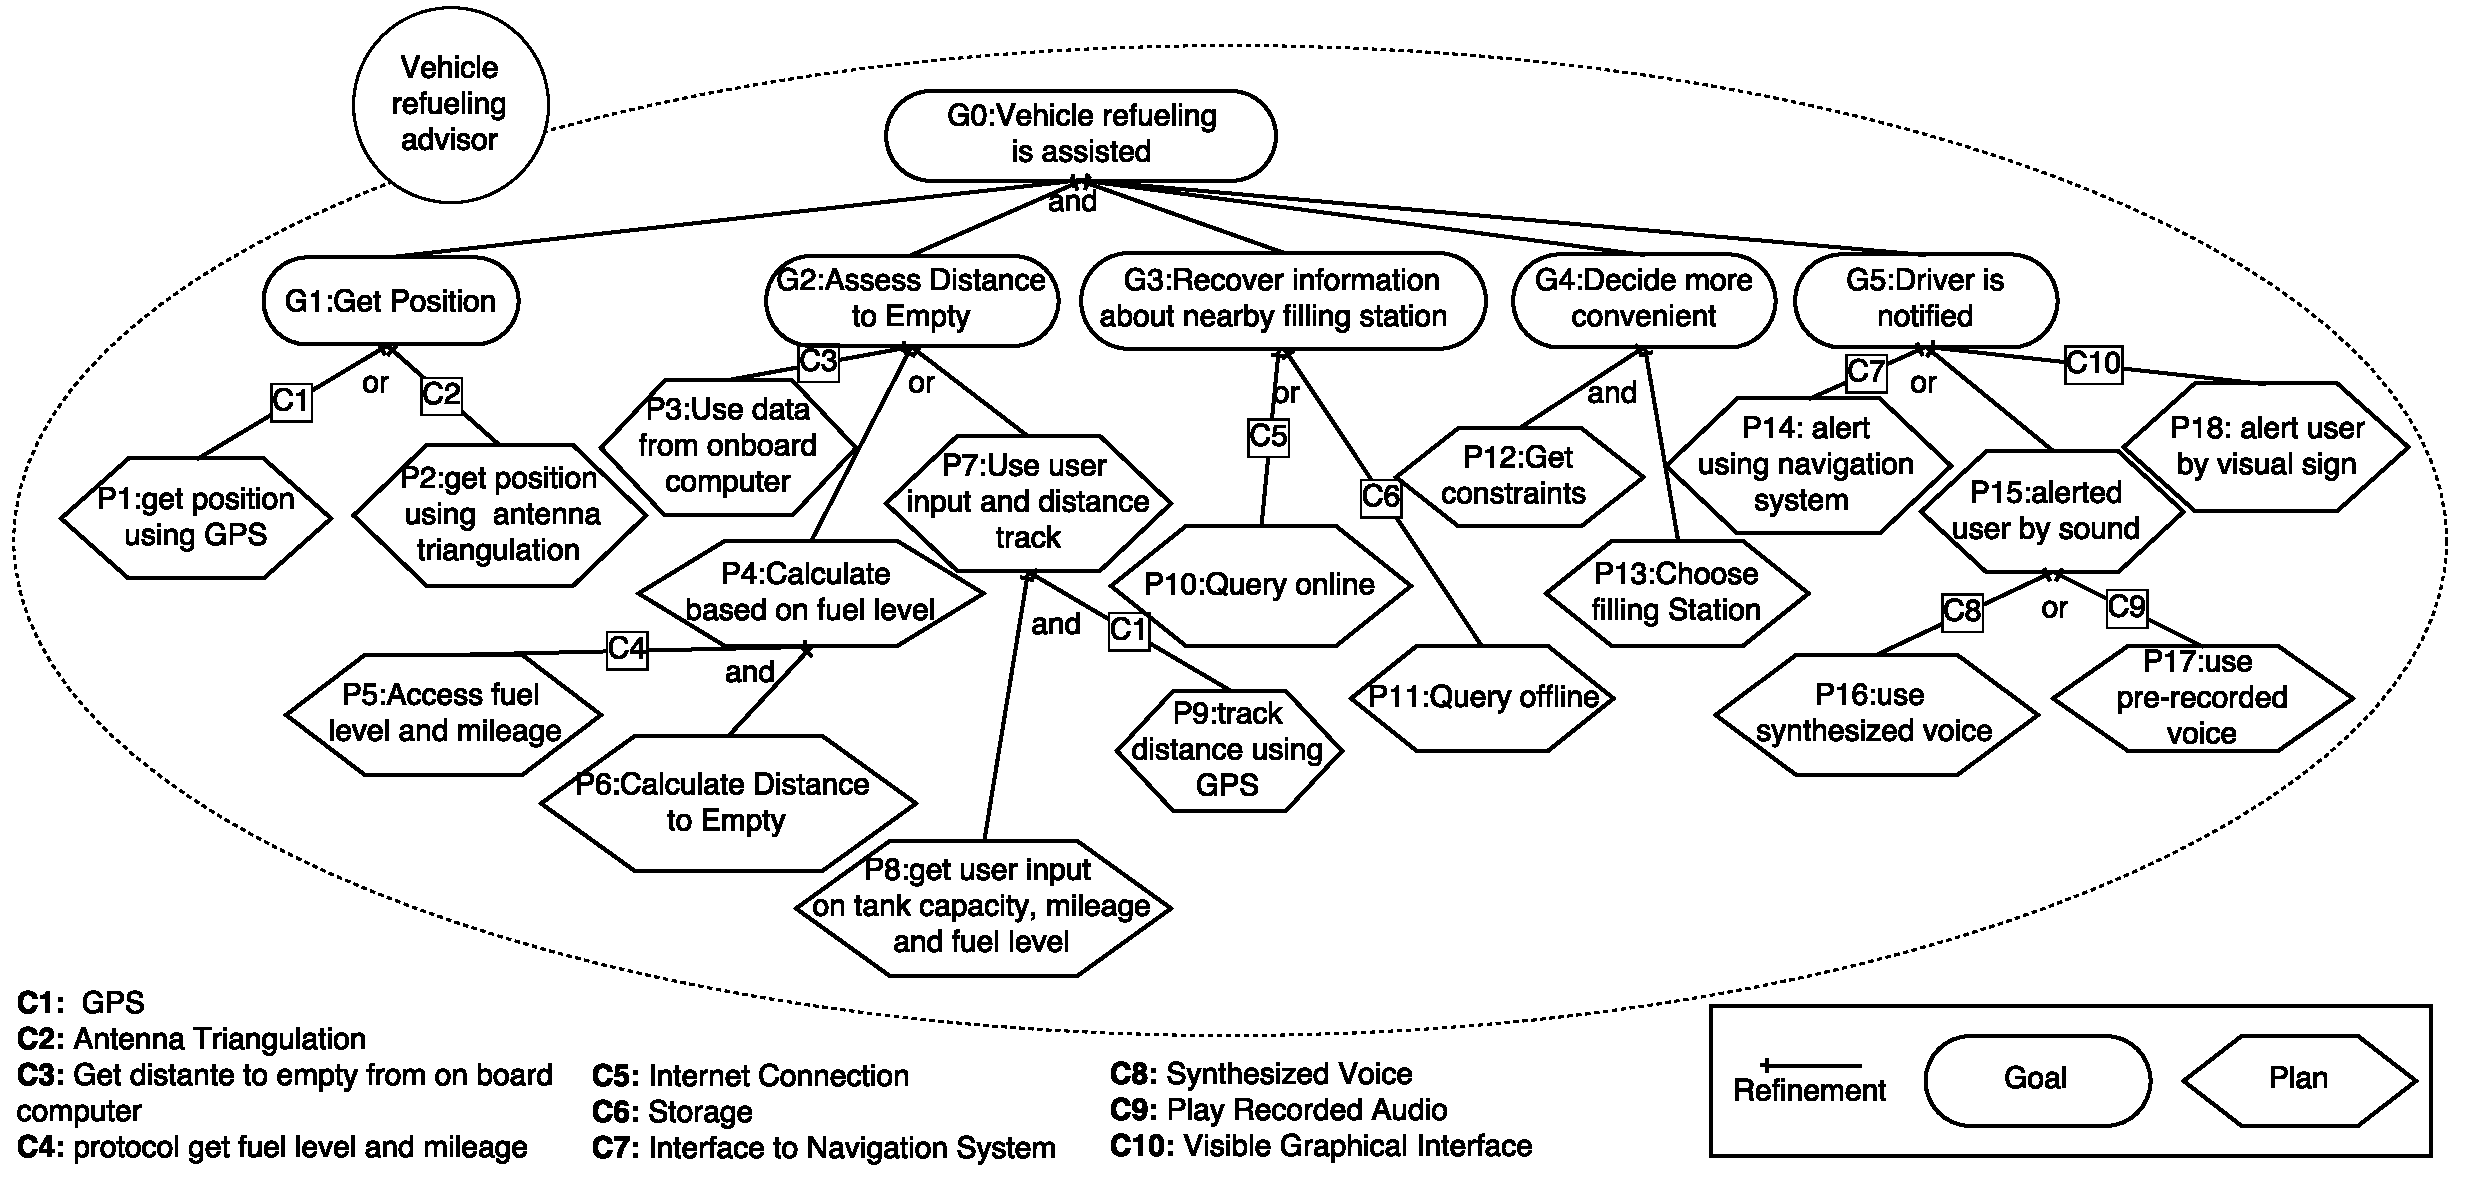
\includegraphics[width=\linewidth]{case_study/goal_model_filling_station_advisor}
 \caption{CGM of the filling station advisor}
\label{fig:goal_model_filling_station_advisor}
\end{figure*}

The CGM presented in Figure~\ref{fig:goal_model_filling_station_advisor} depicts the goals to be achieved by the Filling Station Advisor.
The root objective \emph{G0: Vehicle refueling is assisted} is AND-refined into 5 others objectives G1, G2, G3, G4 and G5. In the Goal modeling semantics it means that in order to achieve the root Goal G0, the agent should achieve the goals G1, G2, G3, G4 and G5.
\emph{G1:Get Position} has a means-end association with P1, P2 and P3. It means that the goal G1 can be achieved by executing that plans. As it is an OR-refinements, it means that G1 can be achieved by successfully executing any of the plans P1, P2 or P3. This OR-refinement introduces a variability to the system, allowing it to achieve to root goals in different ways. The contexts C1 in the association between P1 and G1 means that the Plan P1 is executable if the context C1 holds.
Context conditions on the example are of the type "required context"~\cite{ali_goal-based_2010}. These annotations means that a certain way for achieving (executing) a goal (plan) is applicable if the condition holds for the context.

\begin{figure}[!htb]
 \centering
 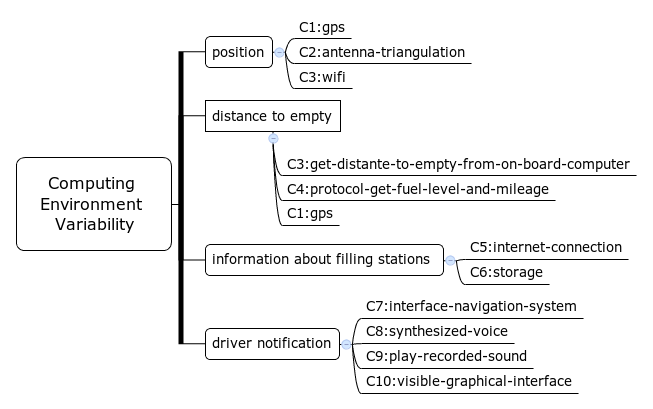
\includegraphics[width=.7\linewidth]{case_study/variability}
 \caption{Variability in the Computing Environment}
\label{fig:variability}
\end{figure}

Figure~\ref{fig:variability} outlines the context space of the target computing environment. It contains variability contexts that are expected to occur in 4 subgoals (G1-G3 and G5) of the application.


\chapter{From Goals To Artifacts}
% Proposal (3.5p)
\label{sec:proposal}


% Gena: Are you really following this approach???
%The rationale behind our approach is the following: an external agent (user or another system) creates a \emph{deployment request}, with goals that should be achieved in a given computing environment. A deployment agent, is responsible to handle that \emph{deployment request} autonomously. The deployment agent is capable of discover available resources in a computing environment it manages. That knowledge about the computing environment is the \emph{context} for the target deployment. The deployment agent is also capable of choosing artifacts from a repository that allows the satisfaction of the deployment request. The process of choosing the correct set of artifacts to allow the deployment request satisfaction is the \emph{deployment planning}.

% General discussion
Following the model proposed by Andersson et al.\cite{andersson_software_2013} for adaptive software development process, we divide our approach into \emph{offline} and \emph{online} activities. In this work, the \emph{offline} activities are conducted by software engineers and result in development and publishing of software components. The \emph{online} activities are autonomously executed in the target environment and result in the deployment of the system. Figure~\ref{fig:overview} presents an overview of the process.

\begin{figure*}[!htb]
  \centering
  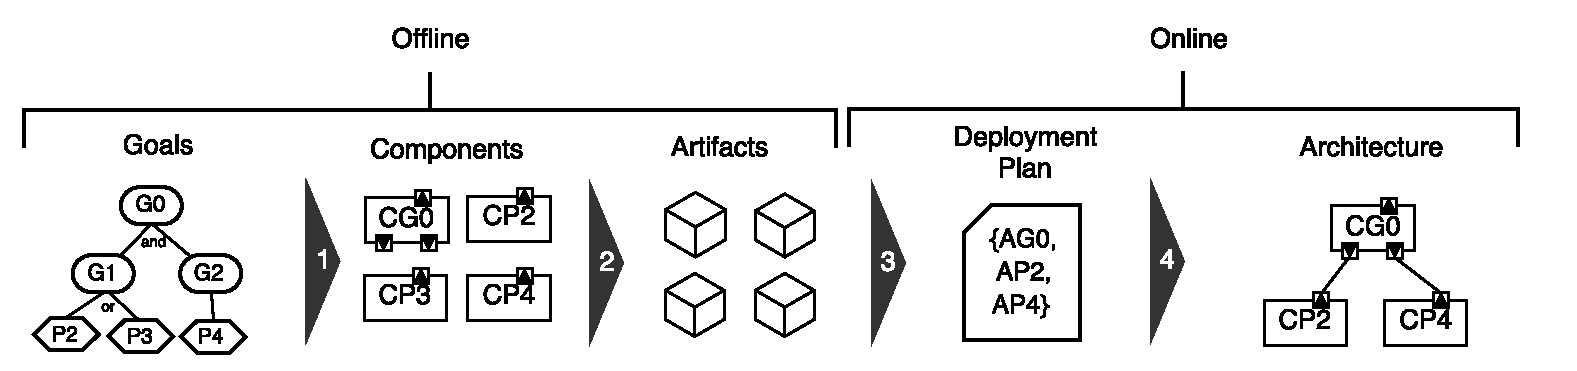
\includegraphics[width=1\linewidth]{transformations}
  \caption{Overview}
\label{fig:overview}
\end{figure*}

Figure~\ref{fig:overview} depicts an overview of the approach, which consists in four major activities: (1) goal modeling, (2) context goal modeling, (3) component analysis and (4) component development. We further explain such activities in details as follows.

In the offline activities, occurs the design of the application. In the first step of our approach, components are mapped from the system CGM using patterns. In the second, these components are packaged into artifacts together with their metadata, which describes what goals the artifact provides, its context conditions and dependencies.
%These packaged artifacts are put in a repository.  Activities: (1) component mapping; \ref{} (2) packaging;\ref{}

In the online part of the approach, the Goalp deployment is autonomously planed in the target computing environment.
The deployment planning is responsible for looking into the repository of artifacts and based on context information and goals, find a set of artifacts that should be deployed to the target computing environment in order to make the goals achievable.
%The deployment planning is detailed in the Section~\ref{sec:planning}. Deployment execution is the last activity and is discussed in Section~\ref{sec:execution}


\section{Offline}

Previously, goal-driven  approaches were proposed for introducing variability at requirements, context modeling, software behavior, and software architecture\cite{angelopoulos_capturing_2015}\cite{yu_goals_2008}.
In our methodology, we propose a systematic approach to support deployment variability, from requirements to deployment.
Deployment variability is important since not taking into account the heterogeneity of a computing environment may lead to unnecessary or even unsuited deployment of components.
Such scenario would bring a negative impact to software performance, or in some cases represent inconsistent deployment of functionalities on the target device.

When developing a monolithic software, we implement in the same codebase all functionalities, then all code is built and deployed together.
In the Filling Station Advisor example, if implementing it as a monolithic software, the logic to get the vehicle position using GPS or antenna triangulation would stay in the same codebase and would be deployed altogether in the target environment, even when it does not have antenna triangulation capability.


In order to better cope with heterogeneity in the computing environment, we should minimize the coupling between parts of the code that have dependencies on specific resources in the environment.
By encapsulating dependencies of specific resources into components, it is possible to create variability at architecture level. By packaging the components into different artifacts, it is possible to maintain such variability at deployment level. Such variability is useful as it allows the deployment of components only to environment that have the required resources.

Regarding the Filling Station Advisor example, depicted in \ref{fig:goal_model_filling_station_advisor}, for goal \emph{G1}(Get Position), components can be implemented providing the actual position of the device by means of GPS or antenna triangulation. These components can be packaged into different artifacts that will only be deployed when the target environment has the appropriate resources.

\subsection{Goal Modelling}
\label{sec:dgm}

A systematic way of analyzing the capabilities of the computing environment is needed in order to support the resolution of variability at deployment-time. First, the available capabilities in the environment should be represented.

\begin{defn}[Resource]

  A resource provides a specific computing capability, it could be available in the computing environment and used in plans. A resource receives a label.

\end{defn}

Each resource relevant to the application receives a label.
Regarding the Filling Station Advisor, examples of relevant resources are \emph{GPS}, (labeled c1) and \emph{antenna triangulation} (labeled c2). Plans can require resources in order to be applicable, for example, \emph{P1: get position using GPS} requires the resource GPS to be available.

In order to reason about available resources in the target computing environment, a context model is used.
In Goalp, the context of a target computing environment is reified as a set of labels.

\begin{defn}[Context]

  A context ctx := r1..rn, \{ r $\in$ ctx | a resource labeled r is available in the target computing environment\}
\end{defn}
The semantics is that if a label is present in the set, the resource is available in the target environment.
In our example, the set [c1, c5, c8] is an example of context, representing that GPS, connection to the Internet and voice synthesizing are resources available in the computing environment.

\begin{defn}[Deployment Goal Model]

  A Deployment Goal Model (DGM) is a tuple (M, ctx\_cond) where:

  \begin{itemize}
    \item M is a design-time goal model \cite{dalpiaz_runtime_2013} defined as a tuple (N, R), where N is a set of goals and plans in the model, and R the corresponding set of relationship links between the elements in N.
    \item ctx\_cond is a context condition associated with a node n $\in$ N. A context condition is associated with a labeled resource, ctx\_cond <> r. is\_satisfied(ctx, ctx\_cond) evaluate a context condition against a context. is\_satisfied(ctx, ctx\_cond):=\texttt{TRUE} iff ctx\_cond <> r, r $\in$ ctx (is\_satisfied resturns TRUE if the resource labeled ctx\_cond  is present in the context)
  \end{itemize}

\end{defn}

\emph{Conditions conditions} represent restrictions to the applicability of a plan. Conditions conditions are represented by labels and are evaluated against a context.
A context condition is satisfied if its associated label is present in the context. For example, in a scenario with context ctx=[c1, c5], the context condition c1 holds while c2 do not.

Context conditions are used to solve variability. In Figure~\ref{fig:goal_model_filling_station_advisor}, the goal \emph{G1:Get position} has two alternatives to be achieved: by executing plan \emph{P1:get position} using GPS or \emph{P2:get position using antenna triangulation}. The plan P1 is applicable if the context condition c1 (GPS) is satisfied, which is the case when GPS capability is available in the target environment.

\subsection{Component Mapping}
\label{sec:goals_components}

Components are architectural units. In our proposal, components definitions are mapped from the CGM and them developed by the architect/developer. That activity is named component analysis. In our vision, components can \emph{provide} goals which means that they can be executed to \emph{fulfill} a goal at runtime.

The patterns present in table~\ref{table_cgm_to_components_patterns} are used, at the component analysis, to map components based on the CGM of the system. By mapping components we mean identifying which component should be developed in order to reflect the CGM of the system. By using the proposed patterns, the variability present in the CGM is kept at the architecture of the system. Theses patterns are an extension of Yu et al.\cite{yu_goals_2008} patterns for the Goals-Component view. We extended Yu et al.\cite{yu_goals_2008} patterns with contextual conditions.

\begin{table}[!htb]
\centering
\caption{Contextual Goal Model to components - patterns}
\label{table_cgm_to_components_patterns}
\bigskip
\begin{tabular}{|c| c p{5cm}|}
\hline
 %\textbf{ A } & \textbf{ B} & \textbf{C} \\ \hline
 And-Refinement &
 \raisebox{-\totalheight}{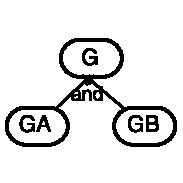
\includegraphics[scale=1]{patterns_and}} &
 \begin{lstlisting}
 Component CG {
   provides IG;
   requires
      IGA, IGB;
 }
 \end{lstlisting} \\ \hline
 Or-Refinement &
 \raisebox{-\totalheight}{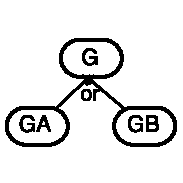
\includegraphics[scale=1]{patterns_or}} &
 \begin{lstlisting}
 Component CG {
   provides IGA;
 }
 Component CG {
   provides IGB;
 }
 \end{lstlisting} \\ \hline
 Context-condition &
 \raisebox{-\totalheight}{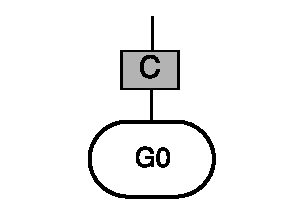
\includegraphics[scale=1]{patterns_condition}} &
 \begin{lstlisting}
 Component CG {
   provides IG;
   condition C;
 }
 \end{lstlisting} \\ \hline
\end{tabular}
\end{table}

The presented patterns for And/Or-refinements and Context-conditions, are described using goals but they can be applied for goals and plans without distinction. Both And/Or-refinements or Goal-Plans means-ends relationship will generate interfaces and components in the same way.

 pattern is applied to plans, as plans are the ones using resources, and being so they are the ones that have restrictions concerning the computing environment.

And-refinements result in components that define a strategy to achieve a given goal by achieving two or more sub, more concrete, goals.
Mapping components from an And-refinemnt results in: (i) a root interface that describe what component provides. (ii) Interfaces for each sub-goal. (iii) A component that provides the root interface and requires each interface generated for sub goals.
Such component implements a strategy to achieve its provided goal. It coordinates the sub more specific goals by calling them and passing one result as the input of another, when applicable.
As an example, applying And-refinement patterns for Root Goal - \emph{G0:Vehicle refueling is assisted} - of the Filling Station Advisor application, will result in interface IG0 and a component G0 that provides IG0 and requires IG1, IG2, IG3, IG4, and IG5.
\begin{lstlisting}
  Component G0 {
    provides IG0;
    requires IG1, IG2, IG3, IG4,IG5;
  }
\end{lstlisting}

Applying Or-refinements patterns results in a root interface definition and in multiple implementations. At the CGM, when Or-refinements are associated with context conditions, it allows for alternative strategies using different resources in the computing environment. Using the association of OR-refinement and context-conditions in the component analysis we preserve the variability present in the CGM into the architecture of the system.

For example, in the Filling Station Advisor, applying the patterns for G1:Get Position, P1:get position using GPS and P2:get position using antenna triangulation will result in the following components:

\begin{lstlisting}
  Component CP1 {
    provides IG1;
    condition C1;
  }
  Component CP2 {
    provides IG1;
    condition C2;
  }
\end{lstlisting}

The two components CP1 and CP2 provides the same goals but have different context conditions (C1:GPS and C2:antenna triangulation). It means that we can achieve the same goal using any of both resource, by deploying one of the two component variants.
That variability in the architecture allows for the adaptation to the heterogeneity in the target environment.

\subsection{Packaging}
\label{sec_artifacts}
\emph{Artifacts} are deployment units.
From the deployment point of view, the components and interfaces should be packaged in a file to be distributed. We name \emph{artifact} as such file.
An artifact should follow a standard packaging schema, so a package manager can manipulate it.
In our approach, we propose to include into the artifact metadata to describe its related goals, context conditions, and dependencies. That metadata reflects information about the packaged components. For our approach, the metadata of interest is the following:

\begin{description}
  \item[Provided goals:] goals that can be made achievable by successfully deploying the component.
  \item[Context conditions:] conditions that can be evaluated against the context. If the conditions are not satisfied it means that the component can not be deployed at the given context. This is the case when the artifact's required resources are not available in the computing environment.
  \item[Dependencies:] required goals that should be provided by other artifacts.
\end{description}

When creating the artifact we can calculate the metadata by looking at the packaged components. The artifact \emph{provided goals} metadata are the union of all \emph{provided goals} of the components packaged in an artifact. The same is valid for \emph{context conditions} and \emph{dependencies} metadata.

Both \emph{context conditions} and \emph{dependencies} impose restrictions on when an artifact can be deployed.
\emph{Context conditions} refer to the need for resources in the computing environment that are beyond the deployment agent capacity of management. Such conditions can be related to hardware implementation, e.g. presence of a GPS-module, our platform lower level software implementation, e.g. access to a protocol to query vehicle onboard computer data. If a context condition does not hold, there is nothing that can be done at deployment time to change that.
\emph{Dependencies}, on the other hand, refer to the need on other artifacts. It is specified in terms of \emph{Provided Goals}. Like other dependency management approaches, an artifact can depend on other artifacts.
Different from other approaches, we specify the dependency not to a specific version of an artifact identification but in terms of what an artifact provides.
In the Filling Station Advisor, the artifact A0, that packs the component G0 depends on IG0-definition and IG0. To satisfy the dependency, an artifacts that provides IG0-definition should be available, as well as at least one artifact that provides IG0. The Figure~\ref{fig:dependency_graph} depicts the dependency relationship between artifacts.

\begin{figure}[!htb]
  \centering
  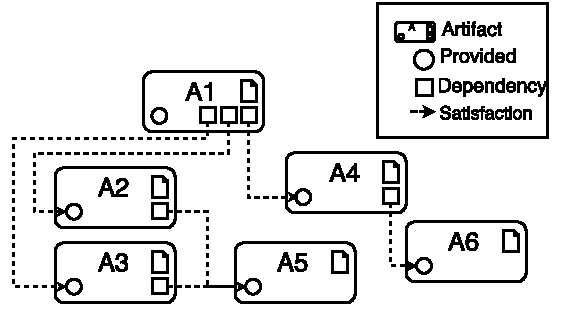
\includegraphics[width=.6\linewidth]{dependency_graph}
  \caption{Dependency Graph}
  \label{fig:dependency_graph}
\end{figure}

Artifacts are registered in a repository which allows the distribution of artifacts to the target environment. In the registration process, the artifact is uploaded to the repository, its metadata is processed, and registered in the repository database.

% Also we have a static dependency between an a component and the interfaces that describes the services it depends on.
% The interfaces and its dependencies (it being clients or implementations) can be packaged separately.
% We have an implementation dependency between a client components and any component that implements the service it depends on. That dependency can be resolved late on, in deployment time.

\subsubsection{Deployment Architectural Style}
\label{depl_arch_style}

In order to maximize the flexibility of systems following Goalp deployment approach, we propose the following architecture style to create artifacts:

Artifacts can be of 3 types:

\begin{description}
  \item[Definition] artifacts that specify the interface of goals. It contains interfaces declarations and data model. It specify the API or contracts for a given set of goals.
  The advantage of separating the goals declaration in a specific artifact is creating implementation independence.
  Goals declarations depends only on other goals declarations and have no context conditions. Goals declarations do not provide any goals.
  % Artifacts providing definitions should be unique in the repository.

  \item[Strategy] artifacts that package components that result from AND-refinements. A Goal refinement provides a high level goal and depends on other more refined goals. It should have no context condition as it do not implement plans that use specific resources in the computing environment.

  \item[Plan implementation] that artifacts contain the domain logic implementation. The plan could have dependencies on specific resources in the computing environment.
  In a dependency tree, artifacts of plan implementation type are the leaves.
  Plan implementation artifacts provides low-level goals and can have dependencies and context conditions.

\end{description}

These types of artifacts are meant to increase the flexibility of deployment.


\subsection{Development Process}

In previous subsections we see the techniques that support the design of software with variability from requirements to deployment. In this section we see how to apply this techniques in a software development process

\subsubsection{Roles}
The proposed process considers three roles: users, requirements engineers and software architects.
Figure~\ref{fig:process_roles} summarizes the collaboration between the roles.

 \begin{figure}[!htb]
   \centering
   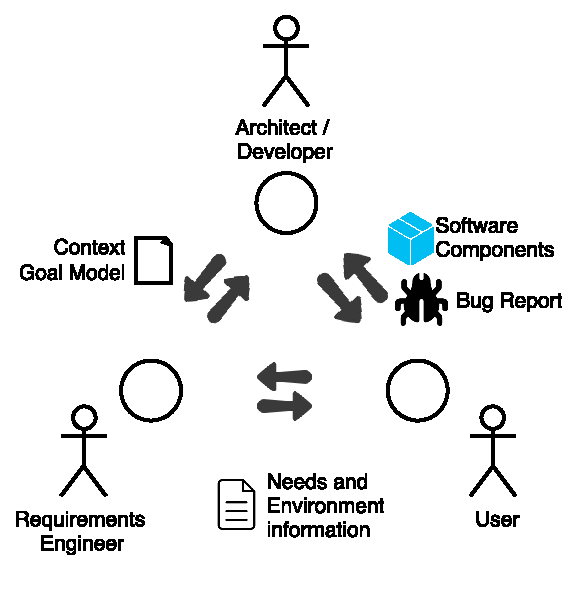
\includegraphics[width=.4\linewidth]{process_roles}
   \caption{Roles collaboration}
 \label{fig:process_roles}
 \end{figure}

\begin{description}
  \item[User]
  This role has access to a particular computing environment and wants to achieve some goals there.
  \item[Requirements Engineer]
  Is responsible for translating users goals to a contextual goal model. Also is responsible for analyzing the different contexts that the system is meant to operate and how they affect the goals.
  \item[Architect] projects the software architecture so as to permit variability of deployment.
  From the point of view of dynamic heterogeneous computing environments, the focus is to create interfaces for components that can allow for goal achievements using different computing resources.

\end{description}



\subsection{Activities}

Figure~\ref{fig:deployment_process_flow} describes the development process activities.

\label{sub:Proposal}
\begin{figure*}[!htb]
  \centering
  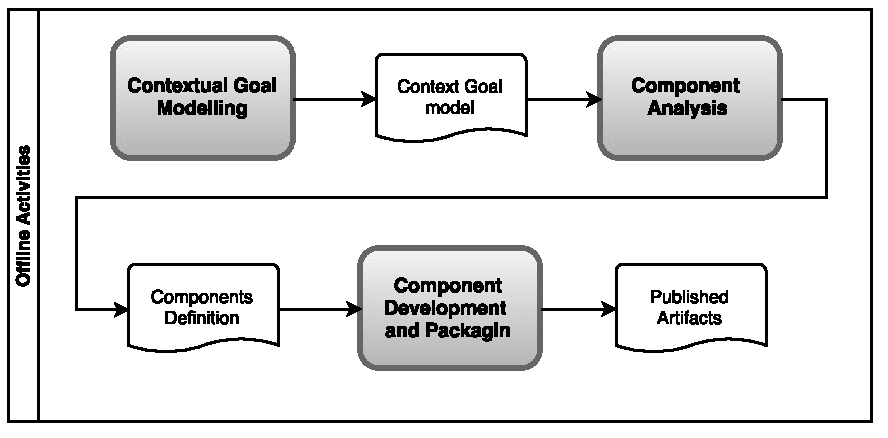
\includegraphics[width=.8\linewidth]{deployment_process_flow}
  \caption{Deployment Process Activities}
\label{fig:deployment_process_flow}
\end{figure*}

\subsubsection{Goal Modeling}
This phase is coordinated by a requirements engineer with the participation of a domain specialist, possibly the user.
In this activity a goal model is created. At the goal model it is identified the solution space, what the system should achieve, and possible strategies to achieve the goals. Also, the goal model creates a common language between users and software engineers.
In this activity, relevant resources should be identified and the goal model should be annotated with \emph{context conditions} related to the computing environment using the formalism described in Section~\ref{sec:dgm}.

\subsubsection{Component Analysis}

The architect is the responsible for this activity. It receives as input a DGM. Then, variability points, components and its interfaces are identified. Component interfaces are created following the guidelines described in Section~\ref{sec:goals_components}.

\subsubsection{Component Development}

The architect is the responsible for this activity. Component development includes the coding, build and test of software components.
Then, components are package into artifacts and put in the repository as described in Section~\ref{sec_artifacts}.


\chapter{Autonomic Deployment Planning}
\section{Autonomic Deployment Planning}
\label{sec:online}

The deployment planning is a online part of the presented approach, executed in the target environment. It is conducted autonomously, using a metamodel and algorithm to come up with a deployment plan.

\begin{figure}[!htb]
  \centering
  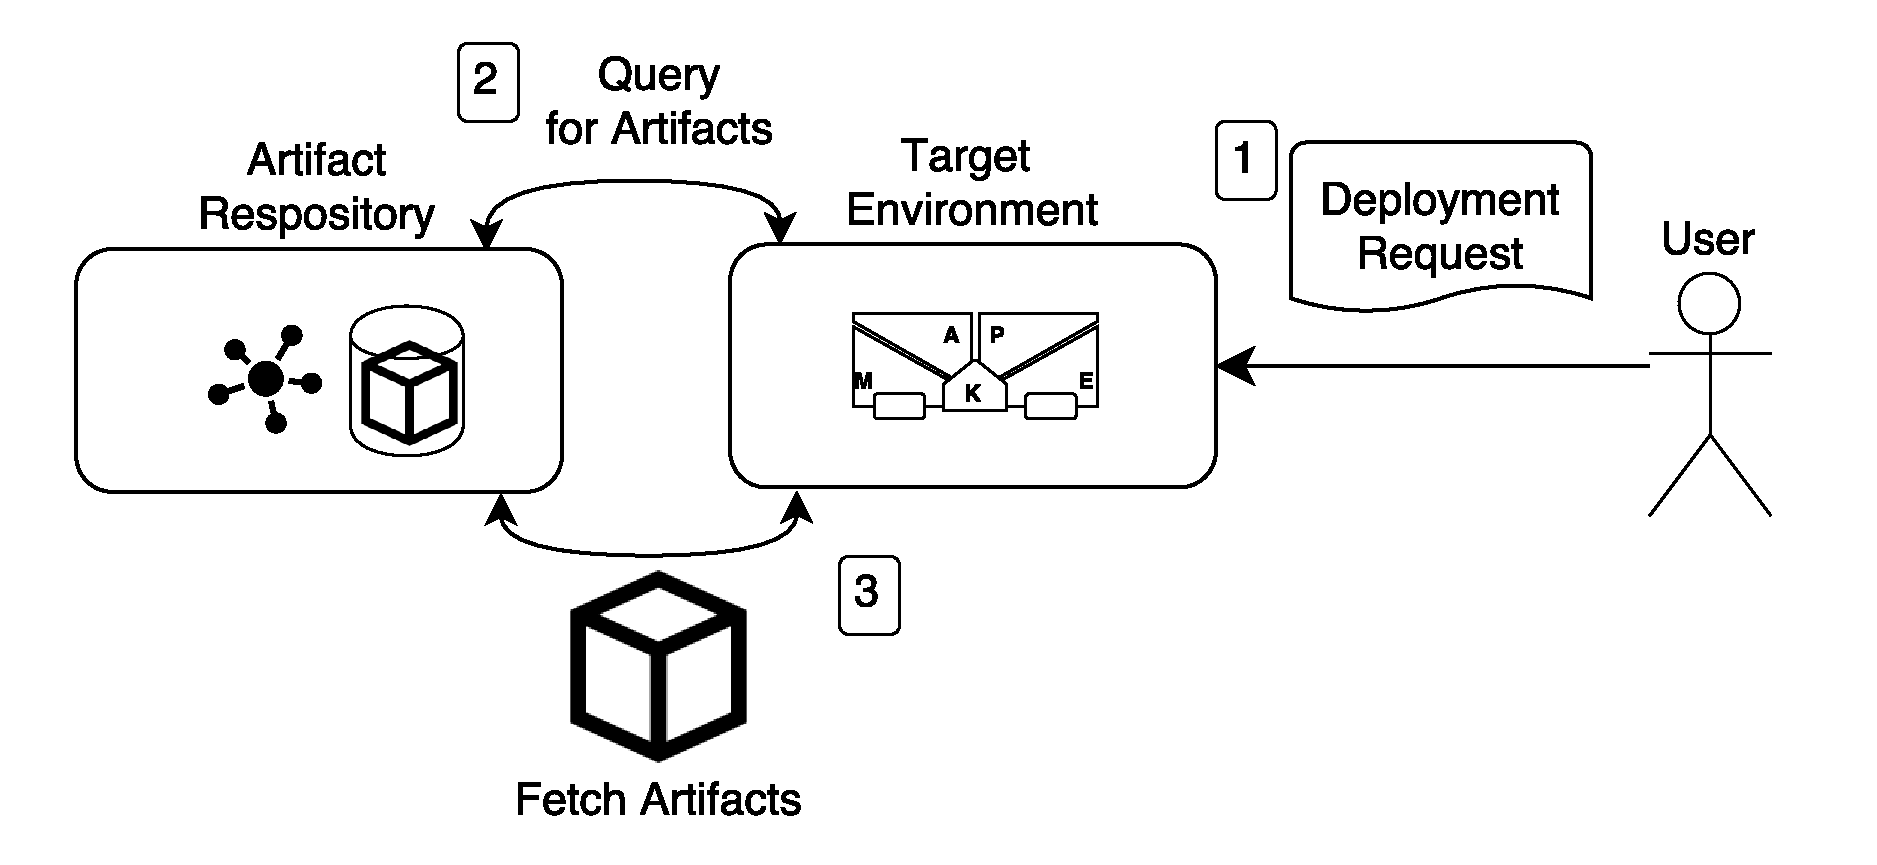
\includegraphics[width=0.5\linewidth]{deployment_actors}
  \caption{Goald Deployment Actors}
\label{fig:deployment_actors}
\end{figure}

Figure~\ref{fig:deployment_actors} depicts the deployment execution. A user interested in using a computing environment to achieve a set of goals submits to this environment which goals it want to achieve in the form of a deployment request.

Then, the system introspect about available computing resources and artifacts present in repository and plan the deployment, generating a deployment plan that is a selection of artifacts that can allow for the goals achievement in the available computing environment. The deployment is them executed by fetching the appropriate artifacts from the repositories.


\section{Deployment Planning}
\label{sec:planning}



\begin{figure}[!htb]
  \centering
  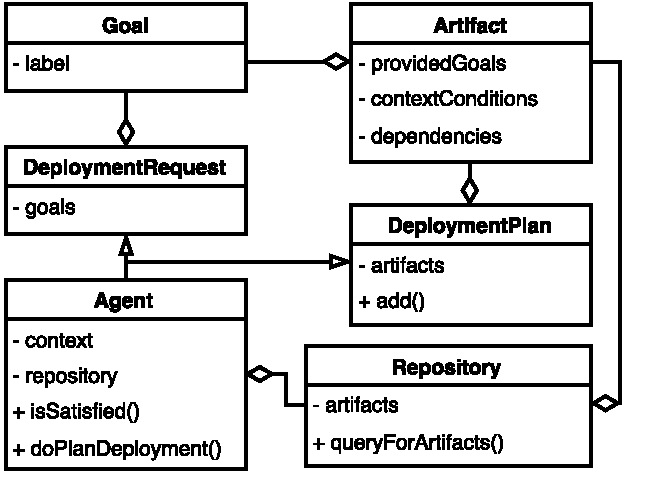
\includegraphics[width=0.5\linewidth]{metamodel}
  \caption{The Goalp Deployment metamodel}
  \label{fig:metamodel}
\end{figure}

Figure~\ref{fig:metamodel} presents the metamodel used. Artifact is the central entity at deployment level. As described in the section~\ref{sec_artifacts}, artifacts has \emph{provided goals}, \emph{context conditions}, and \emph{dependencies}.
Artifacts \emph{provided goals} and \emph{dependencies} create relations of dependency between artifacts, so that an artifact that has a goal dependency is dependent on an artifact that provides that goal. % However, this dependency is loose. An artifact do not depend on one specific other artifact, but instead, on any artifact that provides a goal.

An \emph{agent} can accept deployment requests, action that should trigger the deployment planning. An agent knows a \emph{respository} where it looks for artifacts.
A \emph{repository} has a set of artifacts that it can be queried about by the \emph{queryForArtifacts} method. The method \emph{queryForArtifacts} receives a Goal as argument and return all artifacts in the repository that provide that Goal. An \emph{agent} can verify artifacts \emph{context conditions} satisfaction against its own context by \emph{isSatisfied} method.

The \emph{Deployment Request} is a set of goals that an external entity sent to an agent, requesting it to plan a deployment. The \emph{Deployment Plan} is generated as a result of agent \emph{doPlanDeployment}. The \emph{Deployment Plan} is a set of artifacts that makes the goals specified in the \emph{Deployment Request} achievable.

Note that components do not appear here in this model. Components are architectural units that are packaged into artifacts. The components definitions are mapped and developed by the architect/developer, offline.  And is instantiated and bind by the platform, online. But, it do not appear directly at deployment reasoning, as the abstraction concept at deployment is the artifact.

Artifacts are \emph{deployable} for an agent if all its context conditions and dependencies are satisfiable.
Goals are \emph{achievable} if artifacts that provide that goal are deployable, so there is a \emph{deployment plan} that is able to satisfy this goal.

\begin{figure}[!htb]
  \centering
  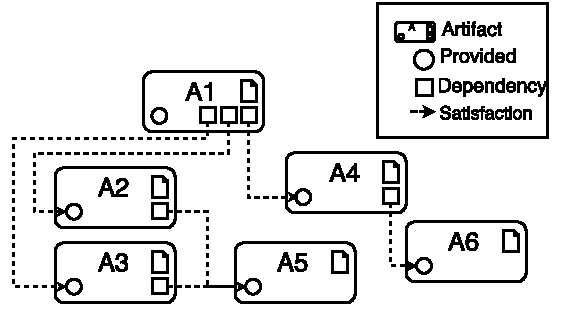
\includegraphics[width=.6\linewidth]{dependency_graph}
  \caption{Dependency Graph}
  \label{fig:dependency_graph}
\end{figure}

% \begin{figure}[!htb]
%   \centering
%   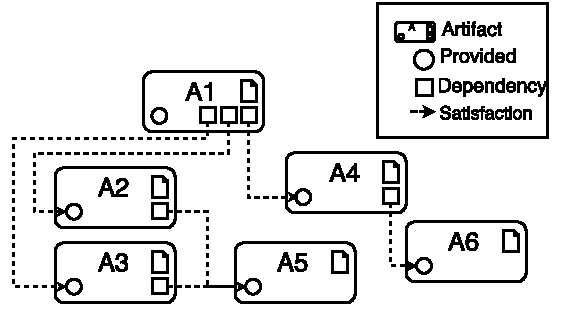
\includegraphics[width=.6\linewidth]{dependency_graph}
%   \caption{Dependency Graph}
% \label{fig:dependency_graph}
% \end{figure}

\subsection{Planning Method}

To come up with a deployment plan for a given a given deployment request and context we present the Algorithm~\ref{plan_method}. It implements the \emph{Agent}'s \emph{doPlanDeployment} method (Figure~\ref{fig:metamodel}).

\begin{algorithm}[!htb]
 \KwIn{DeploymentRequest request}
 \KwResult{DeploymentPlan plan}
  var resultingPlan $\leftarrow$ new DeploymentPlan() \;

  \ForEach{Goal selectedGoal in goals}{
    var subPlan $\leftarrow$ new DeploymentPlan() \;

    var artifacts $\leftarrow$ repository.
    \\queryForArtifacts(selectedGoal) \;

    \ForEach{Artifact artifact in artifacts}{
     	var contextSatisfaction $\leftarrow$ \\
      isSatisfied(artifact.contextConditions)\;

      \If{contextSatisfaction}{
        var plan $\leftarrow$ new DeploymentPlan ()\;

        plan.add(artifact)\;

        \If{artifact.dependencies == EMPTY}{
          subPlan.add(plan)\;

          break\;
        }\Else{
          var depPlan  $\leftarrow$ doPlanDeployment (artifact.dependencies)\;

          \If{depPlan != NULL}{
          plan.add(depPlan)\;

          subPlan.add(plan)\;

          break\;
          }
        }
      }
    }
    \If{subPlan != EMPTY}{
      resultingPlan.add(subPlan)\;

    }\Else{

      \Return{NULL}
    }
  }
  \Return{resultingPlan}

  \caption{doPlanDeployment (List goals)}
  \label{plan_method}
\end{algorithm}

The Algorithm~\ref{plan_method} works as follows: it receives as parameter as deployment request, which contains a list of goals. For each goal in the list, it queries the repository for artifacts that provides this goals (line 4). The repository returns a list of artifacts. For each artifact the algorithm looks for a sub plan with this artifact (line 5-21). First, the context conditions are verified (line 6). If the context is satisfied (line 7),
then a new plan is created with the artifact (line 8-9). If the list of dependencies of the artifact in empty (line 10), them the new plan is added to the sub plan (line 11). Else, if the artifact has a not empty set of dependencies, the algorithm is recursively called for this dependencies. If the results of the recursive call is not NULL (line 15), the resulting plan is added to the new plan and the plan is added to the sub plan (line 16-17).
In both cases that a new plan is added to a sub plan, the look for a deployment plan that satisfy the selected goal is over and the inner for loop is broken (line 12 and 19) and them the sub plan is added to the resulting plan (line 25).
Otherwise, if the context conditions evaluation (line 6) returns FALSE or the recursive call returns NULL, this artifact can not be deployed. The loops continues and others artifacts will be tried. The algorithm tries to come up with a sup plan for the selected goal with another artifact that provides this goal. If after all tries the sub plan is EMPTY (line 27), the deployment for the selected goal is not possible, and the algorithm returns NULL (line 28). Note that the algorithm will return NULL if for any of the goals in the request it is not possible to come up with a plan. Otherwise, the algorithm will return a valid plan.

It could be the case that there are more then one possible valid plan. But this algorithm will return the first one found.  We let for future works the investigation of approaches to come up with the best alternative plan in case that more then one is valid.

\subsection{Verifying a Plan}
\label{verify_plan}

A deployment plan, is valid for a given context if: (i) for each artifact in the plan, for the current context, all context conditions hold.
(ii) for each artifact, for all its dependencies, there is at least one artifact in the plan that provides it (the dependency).

A deployment plan satisfy a deployment request if it valid, and (iii) for each goal, in the deployment request, there is at least one artifact that provides this goal.

Being so, we can verify if a deployment plan satisfy a deployment request by executing the following steps, that verifies the properties (i), (ii) and (iii):

\begin{itemize}
  \item Check if for all selected artifacts, all context conditions are met.
  \item Check if for all selected artifacts, the dependencies are within the deployment plan.
  \item Check if for all goals in the deployment request there are at least one artifacts that declare this goal and one that implements this goal.
\end{itemize}

\subsection{Deployment Execution}
\label{sec:planning}

The last step of the approach is the deployment execution. The deployment execution involves (i) coping the artifacts present in the deployment plan from the repository to the target environment. And (ii) binding the components present into these artifacts, creating the application architecture.

To bind components, the Dependency Injection design pattern can be used. The basic idea of the Dependency Injection, is to have a separate object, an assembler, that wires together client and server components at runtime\cite{fowler_inversion_2004}. The client refers to a component that uses another component (a service) through an interface. The assembler looks for an available service (implementation of the the interface), instantiates it, and wires it into the client object.


%\input{content}
\chapter{Evaluation}
\label{sec:evaluation}

In this chapter, we focus on the evaluation of the proposed approach.
To do so we used the Goal-Question-Metric (GQM) evaluation methodology~\cite{basili_goal_1994}.

Our first evaluation goal G1 is to assess the feasibility of the approach. To do so, we need to evaluate if a software architect/developer can follow the proposed patterns to refine a goal model into components and artifacts. Also, we need to evaluate if the proposed planning algorithm is capable of autonomously creating a reliable deployment plan.
Such an evaluation required the definition of the following questions and metrics:

\begin{itemize}
  \item Q1.1: For the Filling Station Advisor case study, are the goal-component-artifact patterns a feasible approach to map artifacts from the CGM of the case study?
  \begin{itemize}
    \item Accurately maps artifacts for the Filling Station Advisor case study using proposed patterns.
  \end{itemize}

  \item Q1.2: How long would the algorithm take to come up with a deployment plan?
  \begin{itemize}
    \item Time to produce a plan.
  \end{itemize}

  \item Q1.3: How reliable would a plan provided
  by the algorithm be?
  \begin{itemize}
    \item Percentage of correct answers.
  \end{itemize}

\end{itemize}

Since the Filling Station Advisor has a limited size and does not allow for controlled factors experiments, our second goal G2 aims to provide a more comprehensible scalability evaluation of Goalp. So we defined the following questions and metrics:

\begin{itemize}
  \item Q2.1: How does the algorithm scale over the number of artifacts in the deployment plan?
  \begin{itemize}
    \item M2.1: The time consumed to come up with a deployment plan.
  \end{itemize}

  In the context of heterogeneity, we can have many artifacts in the repository that provide the same goal but with different context conditions.
  We named variability level the number of artifacts present in the repository that provide the same goal. It can affect the scalability of the planning because it leads the algorithm to verify alternative dependency trees, which can be computing intensive.

  \item Q2.2: How does the algorithm scale over the variability level on the repository?
  \begin{itemize}
    \item M2.2: The time consumed to come up with a deployment plan.
  \end{itemize}
\end{itemize}

\subsection{Feasibility Assessment}

We validated the feasibility of the approach applying it to the Filling Station Advisor.

The experiments were conducted using a laptop computer with Intel i5-3337U, 12GB DDR3 1600MHz memory, and Linux (Kernel 3.16.0-77generic). OracleJDK(1.8.0 91-b14) was used to build and run the project.
The experiments to evaluate the algorithm correctness
were implemented as automated tests under Java’s JUnit framework.

The code used to execute the evaluation is available on a public repository
\footnote{The evaluation experiments and step by step guide are available at:
\url{https://github.com/lesunb/goalp} Accessed on December 4th, 2016}
as well as the data obtained and scripts used to treat it.
\footnote{The dataset obtained and the R-Script\cite{the_r_foundation_r_2016} used to analyze the dataset is available at:
\url{https://github.com/lesunb/goalp-evaluation/tree/master/scalability/exp2} Accessed on December 4th, 2016}

\emph{Question 1.1, mapping components and artifacts }

We applied the patterns described in Table~\ref{table_cgm_to_components_patterns} to the CGM depicted in Figure~\ref{fig:goal_model_filling_station_advisor}. Then we defined the artifacts that would package that components following the proposed deployment architecture style (\ref{depl_arch_style}). We then mapped 21 different artifacts.

\emph{Question 1.2 and 1.3}

We instantiated an artifact repository with the mapped artifacts. We defined 7 deployment scenarios under different contexts. The scenarios that we used where: (s1) simple phone with ODB2, (s2) smartphone with ODB2, (s3) smartphone without car connection, (s4) dash computer with GPS and no nav sys integration and (s5) dash computer, connected, with GPS and navigation system integration. Scenarios (s6) dash computer without GPS and (s7) nav system without Internet connection or storage are scenarios for which there is no valid deployment plan.

\begin{figure*}[!htb]
 \centering
 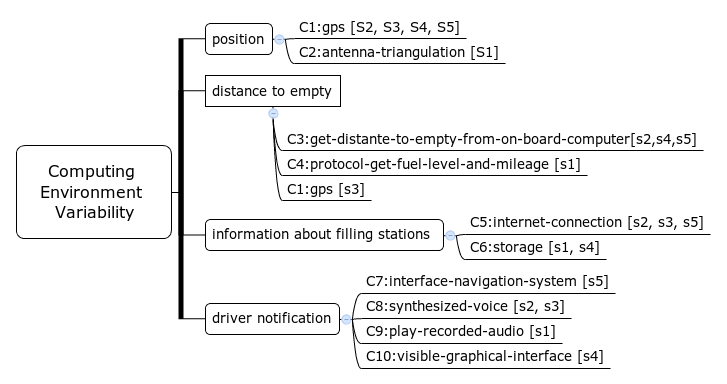
\includegraphics[width=.8\linewidth]{case_study/comp_env_scearios}
 \caption{Computing Environment Evaluation Scenarios}
\label{fig:variability_scenarios}
\end{figure*}

\emph{Question 1.2:  How reliable would a plan provided
by the algorithm be?}: Test cases were created for each scenario (s1-s7).
To validate the algorithm’s correctness,
we verified the generated plans in each test case, asserting if the expected artifacts are in the resulting plan.
For scenarios s1-s5, the planning resulted in valid plans, with the correct artifacts. For scenarios s6 and s7, the algorithm returned \texttt{NULL}, as there is no possible deployment plan for these scenarios.

\begin{figure*}[!htb]
  \centering
  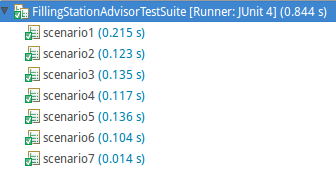
\epsfig{file=results/fsa_testcases, width=3.2in}
  \caption{Passing Tests}
\label{testcase}
\end{figure*}



\emph{Question 1.3: How long would the algorithm take to come up with a deployment plan?}: In each scenario, the time spent by the algorithm was measured. We executed the planning 100 time. Table~\ref{table:planning_time} shows the scenarios, the context, time spent for planning in each scenario, in mile-seconds together with standard deviation.

\begin{table}[!htb]
\centering
\caption{Time to come up with a plan}
\begin{tabular}{|p{0.7cm}|p{3.75cm}|p{2cm}|p{2cm}|}
\hline
  Ref. &
  Context &
  Time (ms) &
  Std \\ \hline

s1 &
C2, C4, C6, C9 &
12.28 ms & 30.69 \\ \hline
s2 &
C1, C3, C5, C8 &
6.24 ms & 16.22 \\ \hline
s3 &
C1, C5, C8 &
9.27 ms & 20.62\\ \hline
s4 &
C1, C3, C6, C10 &
9.01 ms & 20.94 \\ \hline
s5 &
C1, C3, C5, C7 &
6.83 ms & 17.18 \\ \hline
s6 &
C3, C6, C8 &
8.74 ms & 18.76 \\ \hline
s7 &
C1, C3, C7  &
6.44 ms & 17.51 \\ \hline

\end{tabular}
\label{table:planning_time}
\end{table}

    %
    % \item How does it scale over the amount of artifacts in the component repository?
    % \begin{itemize}
    %   \item time to plan the deployment in.
    %   \item space occupied during the planning.
    % \end{itemize}

\subsection{Scalability Assessment}

To evaluate the algorithm's scalability, we developed other test cases.  A repository with randomly generated artifacts was instantiated. And deployment requests that generate plans with a different number of artifacts were made. With this, we could evaluate the impact of the generated plan size in the planning time.
The generated repository had 143,500 artifacts.

The experiments were conducted using a virtual machine in the Azure Cloud. It was used an F1 instance, with 2.4 GHz Intel Xeon® E5-2673 v3 (Haswell) processor,
2GB DDR3 1600MHz memory, and Linux (Kernel 4.4.0-47-generic). OpenJDK(1.9 64bits-build 9) was used to build and run the project.

The code used to execute the evaluation is available on a public repository
\footnote{The needed source code and a step by step guide are available at
\url{https://github.com/lesunb/goalp/tree/master/scalability-evaluation} Accessed on December 4th, 2016}
as well as
the data obtained and scripts used to handle data and plot graphs.
\footnote{R Scripts\cite{the_r_foundation_r_2016} and used dataset are available at
\url{https://github.com/lesunb/goalp/tree/master/scalability-evaluation} Accessed on December 4th, 2016}

\emph{Q2.1: How does the algorithm scale over the number of artifacts in the deployment plan?} We executed 100 deployment planning requests, with different levels of complexity, where the generated plans were composed of artifacts summing from 40 to 3,100 artifacts.

\begin{figure}[!htb]
  \centering
  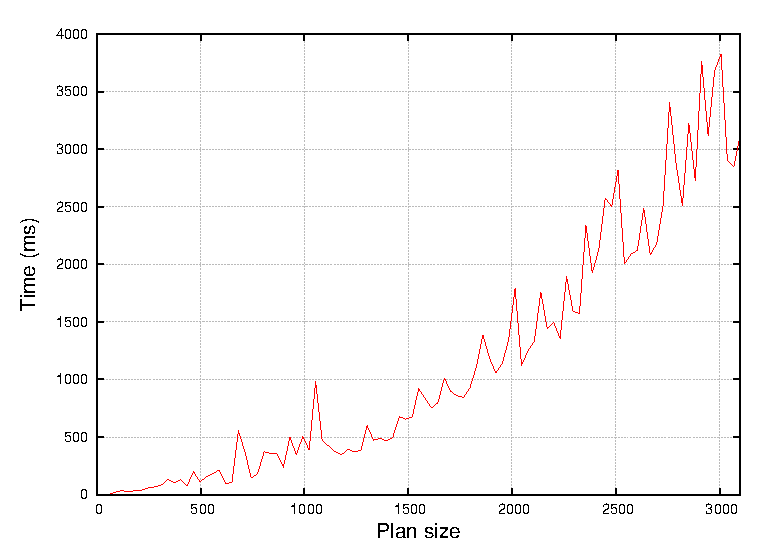
\epsfig{file=results/planning/plan_size_vs_time.eps, width=5.2in}
  \caption{Scalability over the size of plan}
\label{graph_plan_size_and_time}
\end{figure}

The observed time in function on the number of artifacts in the plan is shown in Figure~\ref{graph_plan_size_and_time}.

\emph{Q2.2:  How does the algorithm scale over the variability level on the repository?}
We repeated the experiment for different levels of variability in the repository, from 1 to 10. A variability level of 1 being so that for each plan implementation there was just one artifact that implement the plan. While in variability level 2, for each plan implementation there was two artifacts, and so on.

The result is depicted in Figure~\ref{graph_scalability}. Each curve represents a different level of variability.

\begin{figure}[!htb]
  \centering
  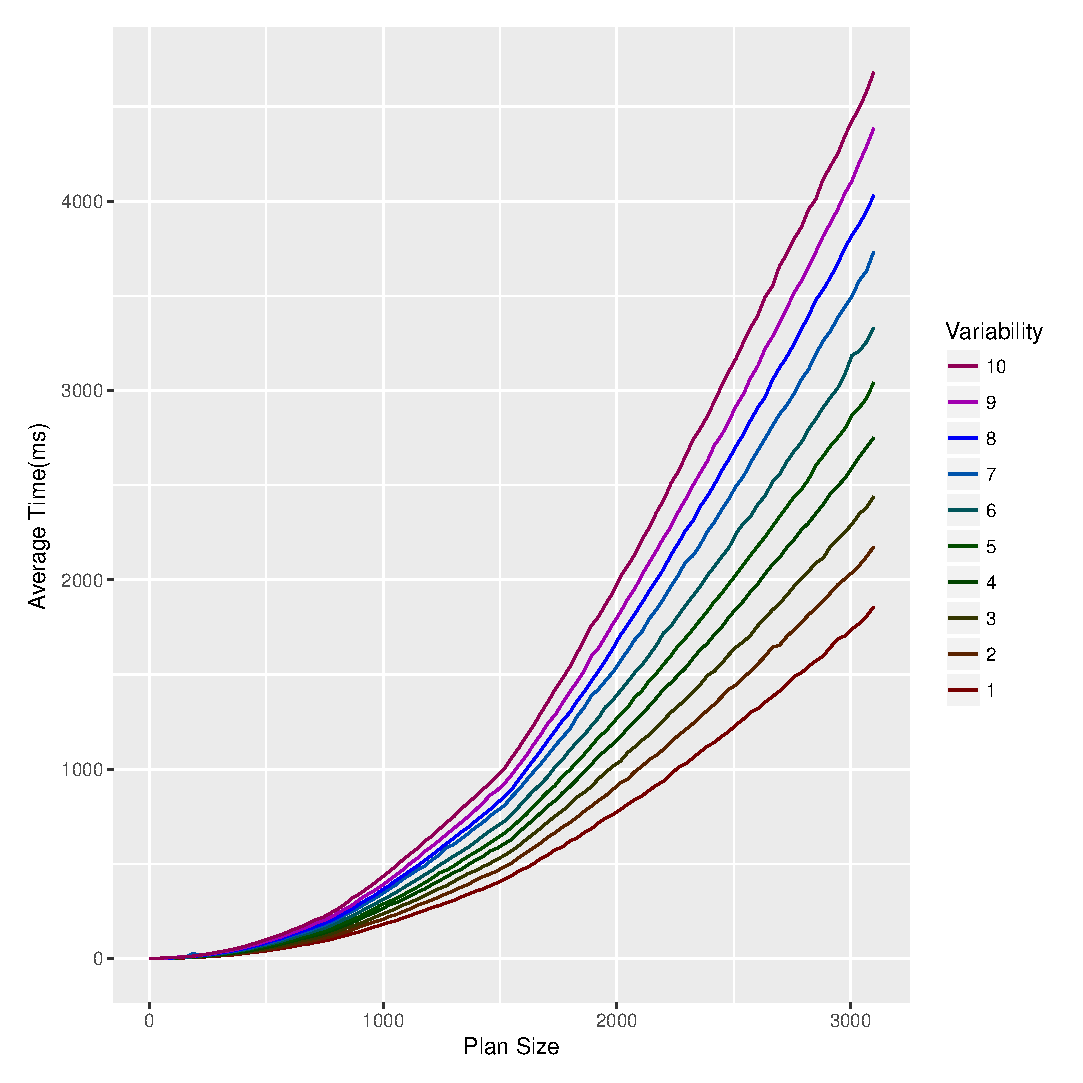
\epsfig{file=results/planning/size_and_variability.eps, width=5.2in}
  \caption{Scalability over variability level - Average (10 executions)}
\label{graph_scalability}
\end{figure}

At the worst case, a deployment request that needs 3,100 artifacts, with 10 variants for each artifact, took less than 5s to be planned. Requests that required up to 1,000 artifacts could be fulfilled in less then a half-second.

\subsection{Discussion of Results}

In conclusion, the time spent planning the deployment is expected to be negligible in face the time that would take to copy the artifacts from a repository to the target environment.

%\section{Evaluation}
\chapter{Conclusion}
%Conclusions(0.75p)
\section{Conclusion and future work}
\label{sec:conclusion}

% TODO relate with multi-level adaptation.
In this paper we presented Goalp, a novel approach to tackle deployment in highly heterogeneous computing environments.
Goalp allows systems deployment to heterogeneous environments, partially unknown at design-time, without requiring a system administrator.
Goalp consists in support to design a system with the needed variability to handle the heterogeneity, from requirements, through architecture, and deployment.
And in online support for solve the variability at deployment time, finding the correct set of artifacts that allows the user achieve its goals in a given target computing environment. Goalp uses a CGM to specify variability at requirements. Further, patterns are used to map components from the CGM and keep the variability are architecture level, and deployment level. The novelty of our approach is that we provide a systematic way to design a system with focus in variability form requirements to deployment.
% As such, using a goal-oriented approach to deployment is expected to integrate with other approach that handle variability in another level.

Following our approach the system implemented reflects the goal-model, keeping the goals traceable to components and artifacts. Via such traceability the adequate set of artifacts is autonomously chosen achieving the target software goal in a given computing environment. Since goal-models are highly abstract models, using it to drive the system adaptation, we expect to achieve a higher level of flexibility transcending the lower-level abstraction computing layers. In addition, by using context-goal models, we can handle computing resources variability. By using CGM for deployment, rework is avoided, as CGM is a model already developed in the requirements elicitation stage.

In a preliminary evaluation, we applied the Goalp approach in a case study. Further, we evaluated the scalability of the algorithm when planning in a large scenario, using a randomly generated repository and deployment requests. The results shows that the algorithm is capable of come up with a plan, in a reasonably large scenario in seconds.

This work fits in our long term vision of a method for design systems with variability at all stages of system design, from requirements to deployment. And a self-adaptable platform that can adapts the software deployment in order to make high-level user goals achievable. This work fits in this vision by providing the knowledge and planning part in a MAPE-K\cite{kephart_vision_2003} architecture.
For future work, we plan to: (1) extend Goalp with deployment planning for multiple nodes by including delegation as another form of variability;  (2) evolve Goalp deployment planning in a self-adaptive approach for deployment, based on MAPE-K, with addition of monitoring, analyzing, and executing capabilities; (3) evaluate Goalp in a open adaptation scenario with multiple developers providing components to the environment; and (4) evaluate self-adaptation at deployment level as a method of fault-tolerance that adapts the system deployment in response to failures in resources.
%We provide a approach that To the best of our knowledge no other approach has tackle this problem.
%We believe that this is will be useful in domain such as ubiquitous at where no specialized people interact with the system and would like it to adapt its deployment.

%The advantages of goal-driven is:
%High level of flexbility by using the system goals as a model for evaluate alternatives of adaptation.
%Easy the development by reuse the goal model.
%The advantages of using a MAS approach is the distributed nature of the system and to avoid have a sigle point of failure.

%\section{Conclusion}

\postextual
\anexos


\bibliographystyle{plain}
\bibliography{bibliografia}
\end{document}
